\documentclass[8pt]{beamer}
\usepackage[T1]{fontenc}
\usepackage[francais]{babel}
\usepackage{tikz}
\usetikzlibrary{arrows,shapes}
\usepackage{pslatex}
\usepackage{textcomp}
\usepackage[utf8]{inputenc}
\usepackage{wrapfig}
\usepackage{graphicx}
\usepackage[section]{placeins}
\usepackage{lscape}
\usepackage{float}
\usepackage{amssymb}
\usepackage{wasysym}
\usepackage{pgf}
\usepackage{alltt}
\usepackage{eso-pic}
\usepackage{url}
\usepackage{tikz}
\usepackage{listings}
\usepackage{color}
\definecolor{mymauve}{rgb}{0.58,0,0.82}

\lstset{language=C++,
basicstyle=\footnotesize,
keywordstyle=\color{red}\bfseries,
breaklines=true,
commentstyle=\color{blue},
stringstyle=\color{mymauve},
literate={ô}{{\^o}}1 {é}{{\'e}}1 {à}{{\`a}}1 {è}{{\`e}}1 {î}{{\^{\i}}}1 {ê}{{\^e}}1 {ç}{{\c c}}1,
morekeywords={string,fstream,ofstream,ifstream}
}
\usepackage{hyperref}

%\hypersetup{urlcolor=blue}

\usetheme{CambridgeUS}


\title[DQM4HEP - v04-02-00]{Data Quality Monitoring for High Energy Physics (DQM4HEP) \\ Version 04-02-00}
\institute[UCBL - IPNL - UGent]{Université Claude Bernard Lyon 1 - Institut de Physique Nucléaire de Lyon / Ghent University}
\author[Eté - Pingault - Mirabito]{{\bf \large R. \'Eté, A. Pingault, L. Mirabito}}
\date{\today}

\DeclareUnicodeCharacter{00A0}{ }

\setbeamertemplate{itemize items}[ball]
\definecolor{MyGreen}{rgb}{0.1,0.5,0.1}
\setbeamercolor{structure}{fg=red!70!black}
\setbeamercolor{block title}{bg=red!70!black,fg=black}
\addtobeamertemplate{block begin}{\pgfsetfillopacity{0.5}}{\pgfsetfillopacity{1}}

\begin{document}


  %%%%%%%%%%%%%% Page de présentation %%%%%%%%%%%%%%
  \begin{frame}

    \titlepage
    \begin{center}
      
\includegraphics[width=0.5\textwidth]{logo/logo-ucbl-ipnl.jpg} ~~~~~~~~~~~
      
\includegraphics[width=0.2\textwidth]{logo/Ghent_University_logo.png}
    \end{center}
  \end{frame}

  \begin{frame}
    \tableofcontents
  \end{frame}


  %% OVERVIEW %%
   \section{Overview and packaging}


  %% GENERAL %%
  \begin{frame}
    \frametitle{\secname}
    \framesubtitle{DQM4HEP : an online monitoring system for data quality}

    \begin{block}{Key points}
      \begin{itemize}
        \item Event distributed system : server/client paradigm
        \item Set of interfaces for data analysis, adapted to DQM purpose
        \item Histogram distributed system
        \item Visualization interface (Qt GUI)
        \item Large scale remote process management
        \item Generic IO support for any edm (opt. LCIO)
        \item Full size HEP experiment to single detector prototype design
        \item ELog interface
      \end{itemize}
    \end{block}
    ~ \\
    Set of interfaces inspired from CMS DQM system (monitor elements, collectors). \\
    ~ \\
    Application flow inspired from ALICE DQM system, AMORE (cycles).

  \end{frame}


  %% PACKAGES %%
  \begin{frame}
    \frametitle{\secname}
    \framesubtitle{DQM4HEP packages}

    One location : \href{https://github.com/DQM4HEP}{\tt https://github.com/DQM4HEP} \\
    Webpage : \href{dqm4hep.github.io}{\tt dqm4hep.github.io} \\
    \begin{block}{The main package : DQM4HEP}
      Installation package for sub-packages (CMake). \\
      Sub-packages :
      \begin{itemize}
        \item \textbf{dim} : Distributed Information Management (Delphi). Manage client/server communications
        \item \textbf{dimjc} : DIM Job Control (L. Mirabito). Remote process management using dim.
        \item \textbf{jsoncpp} : Json I/O for dimjc
        \item \textbf{streamlog} : logging library (used in ILCSOFT)
        \item \textbf{DQMCore} : Core part of the DQM system. Client/server interfaces, analysis, IO, run control interface, plugin management ...
        \item \textbf{DQMViz} : Qt visualization interfaces. Job control gui client, monitoring gui client, run control server gui (standalone).
        \item \textbf{LCIO} : Linear Collider IO. Build support for LCIO streamer
      \end{itemize}
      Forseen packages :
      \begin{itemize}
        \item \textbf{xdrstream} : Generic Xdr serializer
        \item \textbf{xdrlcio} : Lcio serialization using xdrstream (buffer -> socket)
        \item \textbf{DQM4ILC} : ILC specific implementation (detector prototypes modules, marlin helper, ...)
      \end{itemize}
    \end{block}

  \end{frame}


  %% INSTALLATION %%
  \begin{frame}
    \frametitle{\secname}
    \framesubtitle{Installation}

    \begin{block}{Installation mode}
      ~ \\
      Designed to be built \textbf{standalone} or using \textbf{ILCSOFT}. \\
      Basic install requires ROOT. \\
      Full install with DQMViz requires Qt and ROOT \textbf{compiled with \textit{--enable-qt} option}. \\
      ~ \\
      \underline{Standalone mode} :
      \begin{itemize}
        \item Basic install : dim, dimjc, jsoncpp, streamlog, DQMCore
        \item Full install : + DQMViz, LCIO
      \end{itemize}
      ~ \\
      \underline{ILCSOFT mode} :
      \begin{itemize}
        \item Basic install : dim, dimjc, jsoncpp, DQMCore
        \item Full install : + DQMViz
      \end{itemize}
    \end{block}
  \end{frame}



  \section{Architecture and API}

  %% Architecture %%
  \begin{frame}
    \frametitle{\secname}
    \framesubtitle{Global workflow}

    \begin{center}
      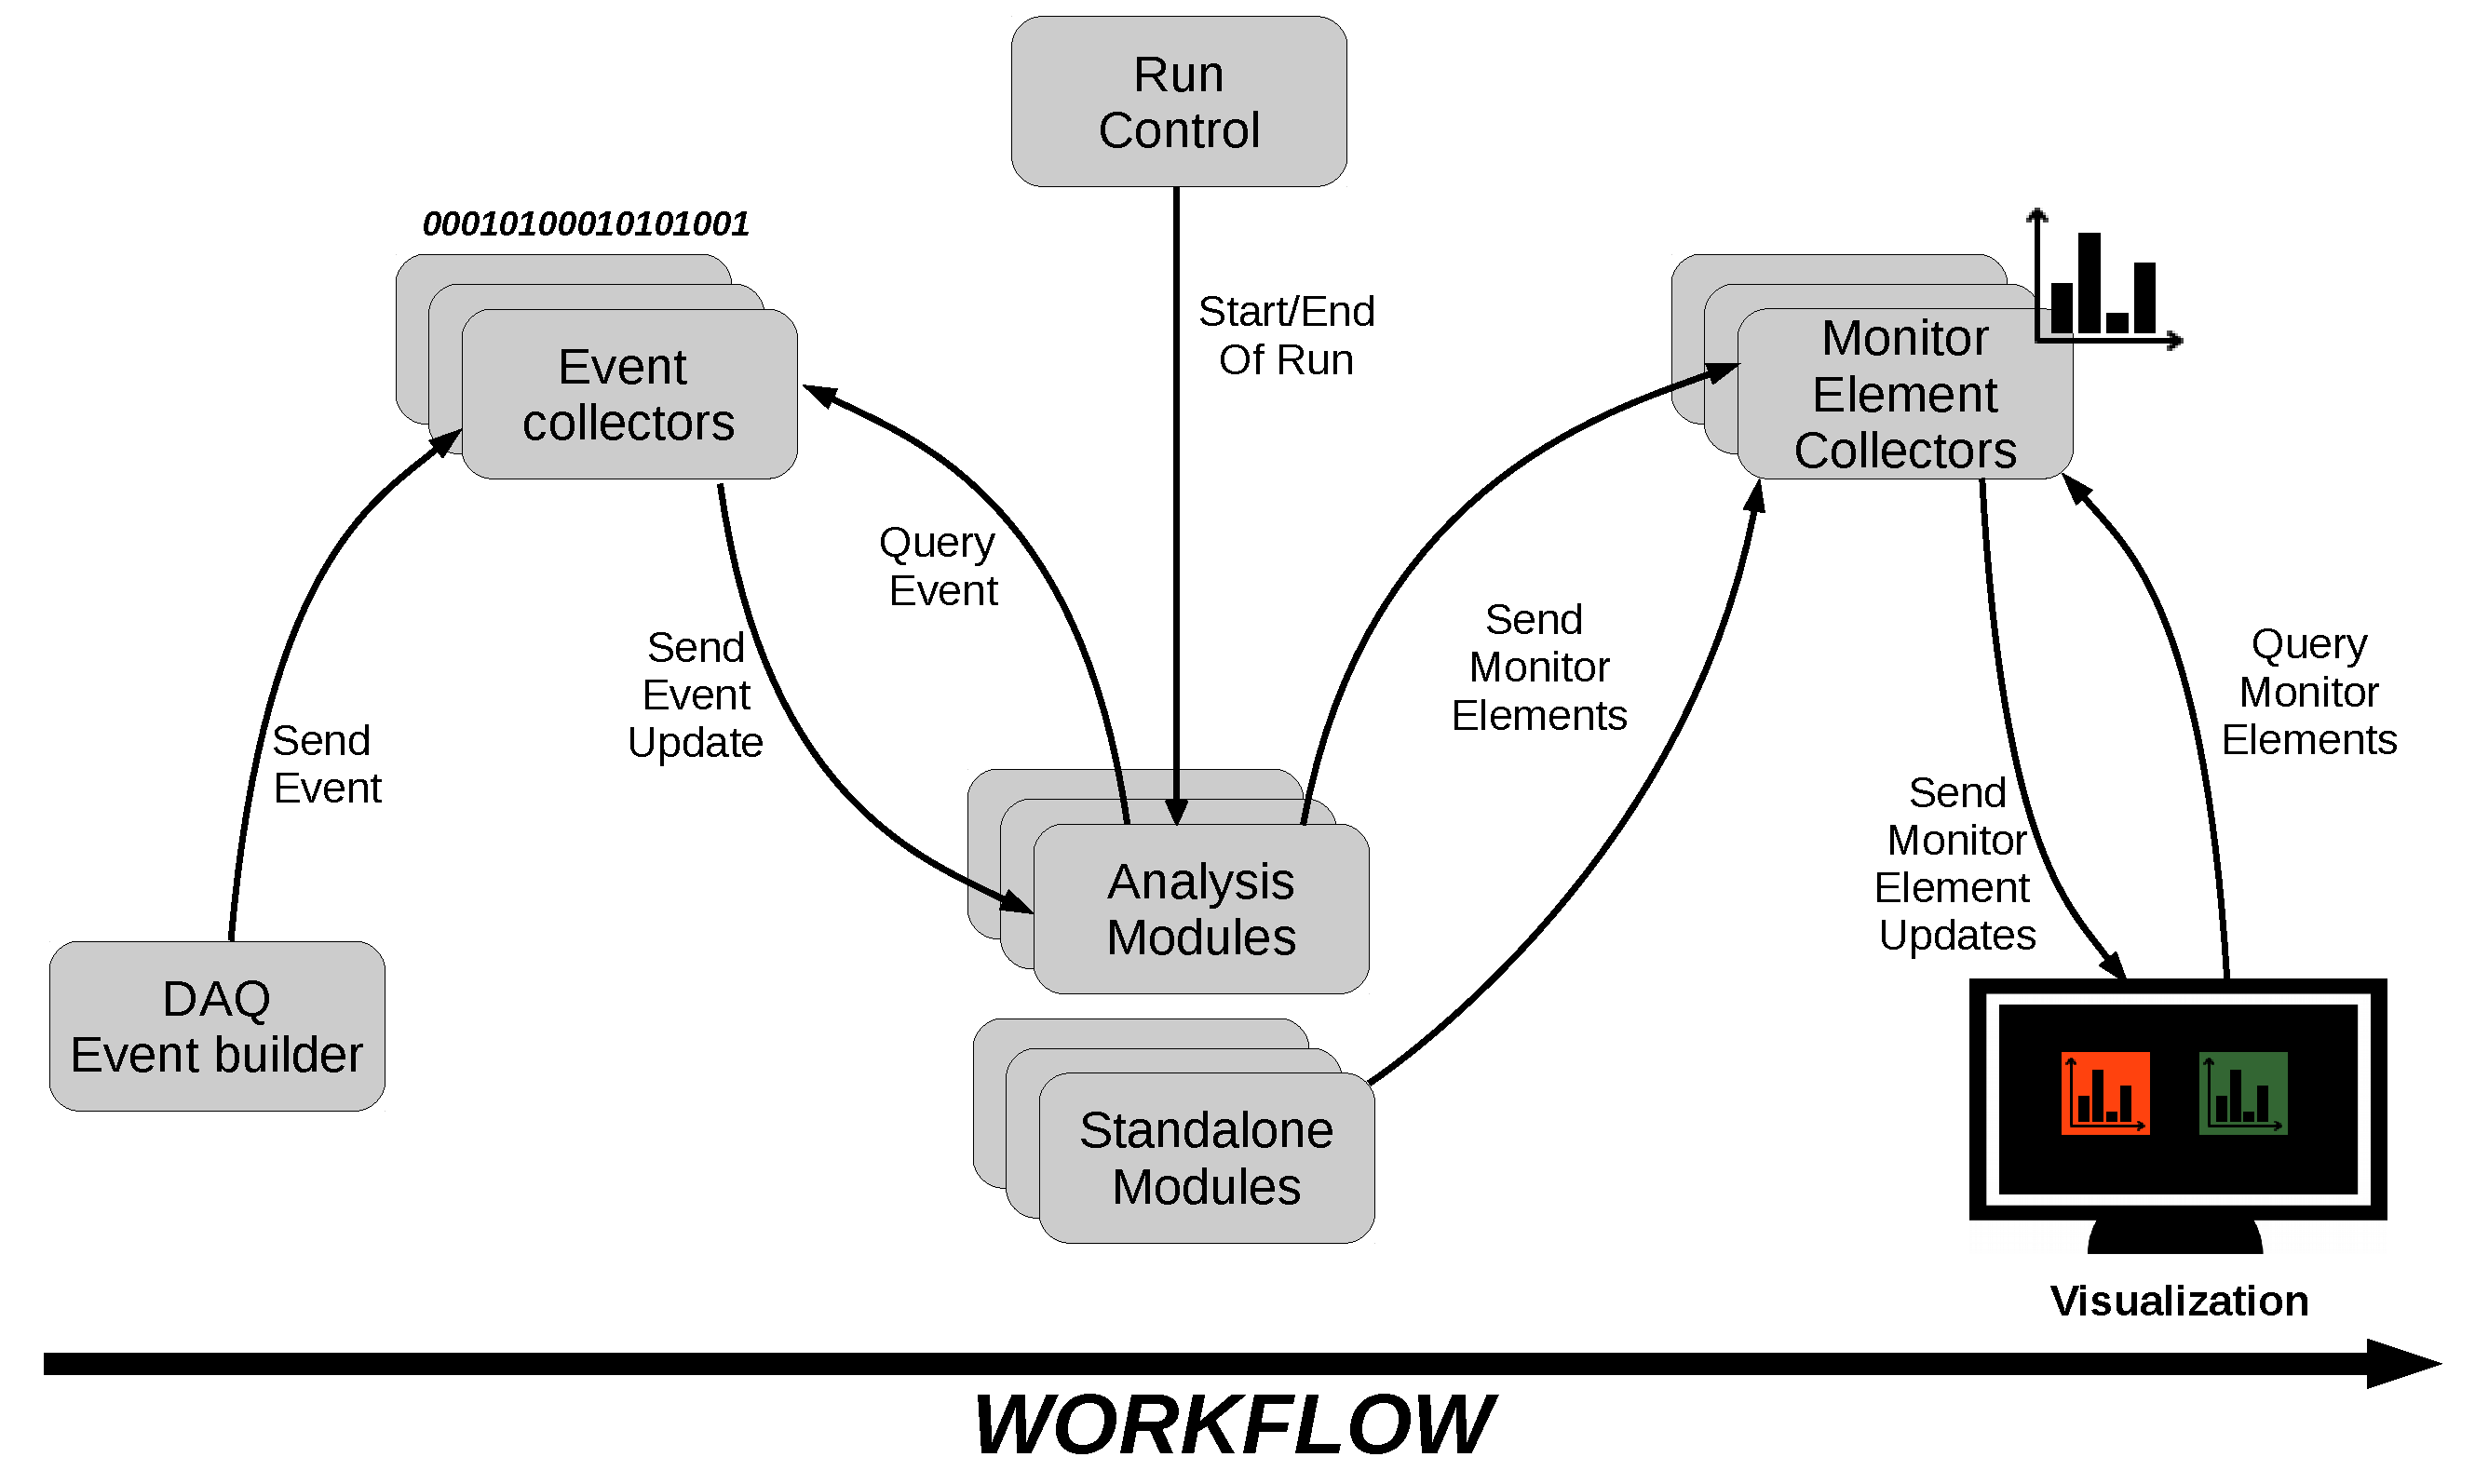
\includegraphics[width=\textwidth]{figs/DQM4HEP_workflow.pdf}
    \end{center}

  \end{frame}




    %% SDHCAL DAQ %%
    \begin{frame}
      \frametitle{\secname}
      \framesubtitle{DAQ interface example : SDHCAL DAQ interface}
      \begin{center}
        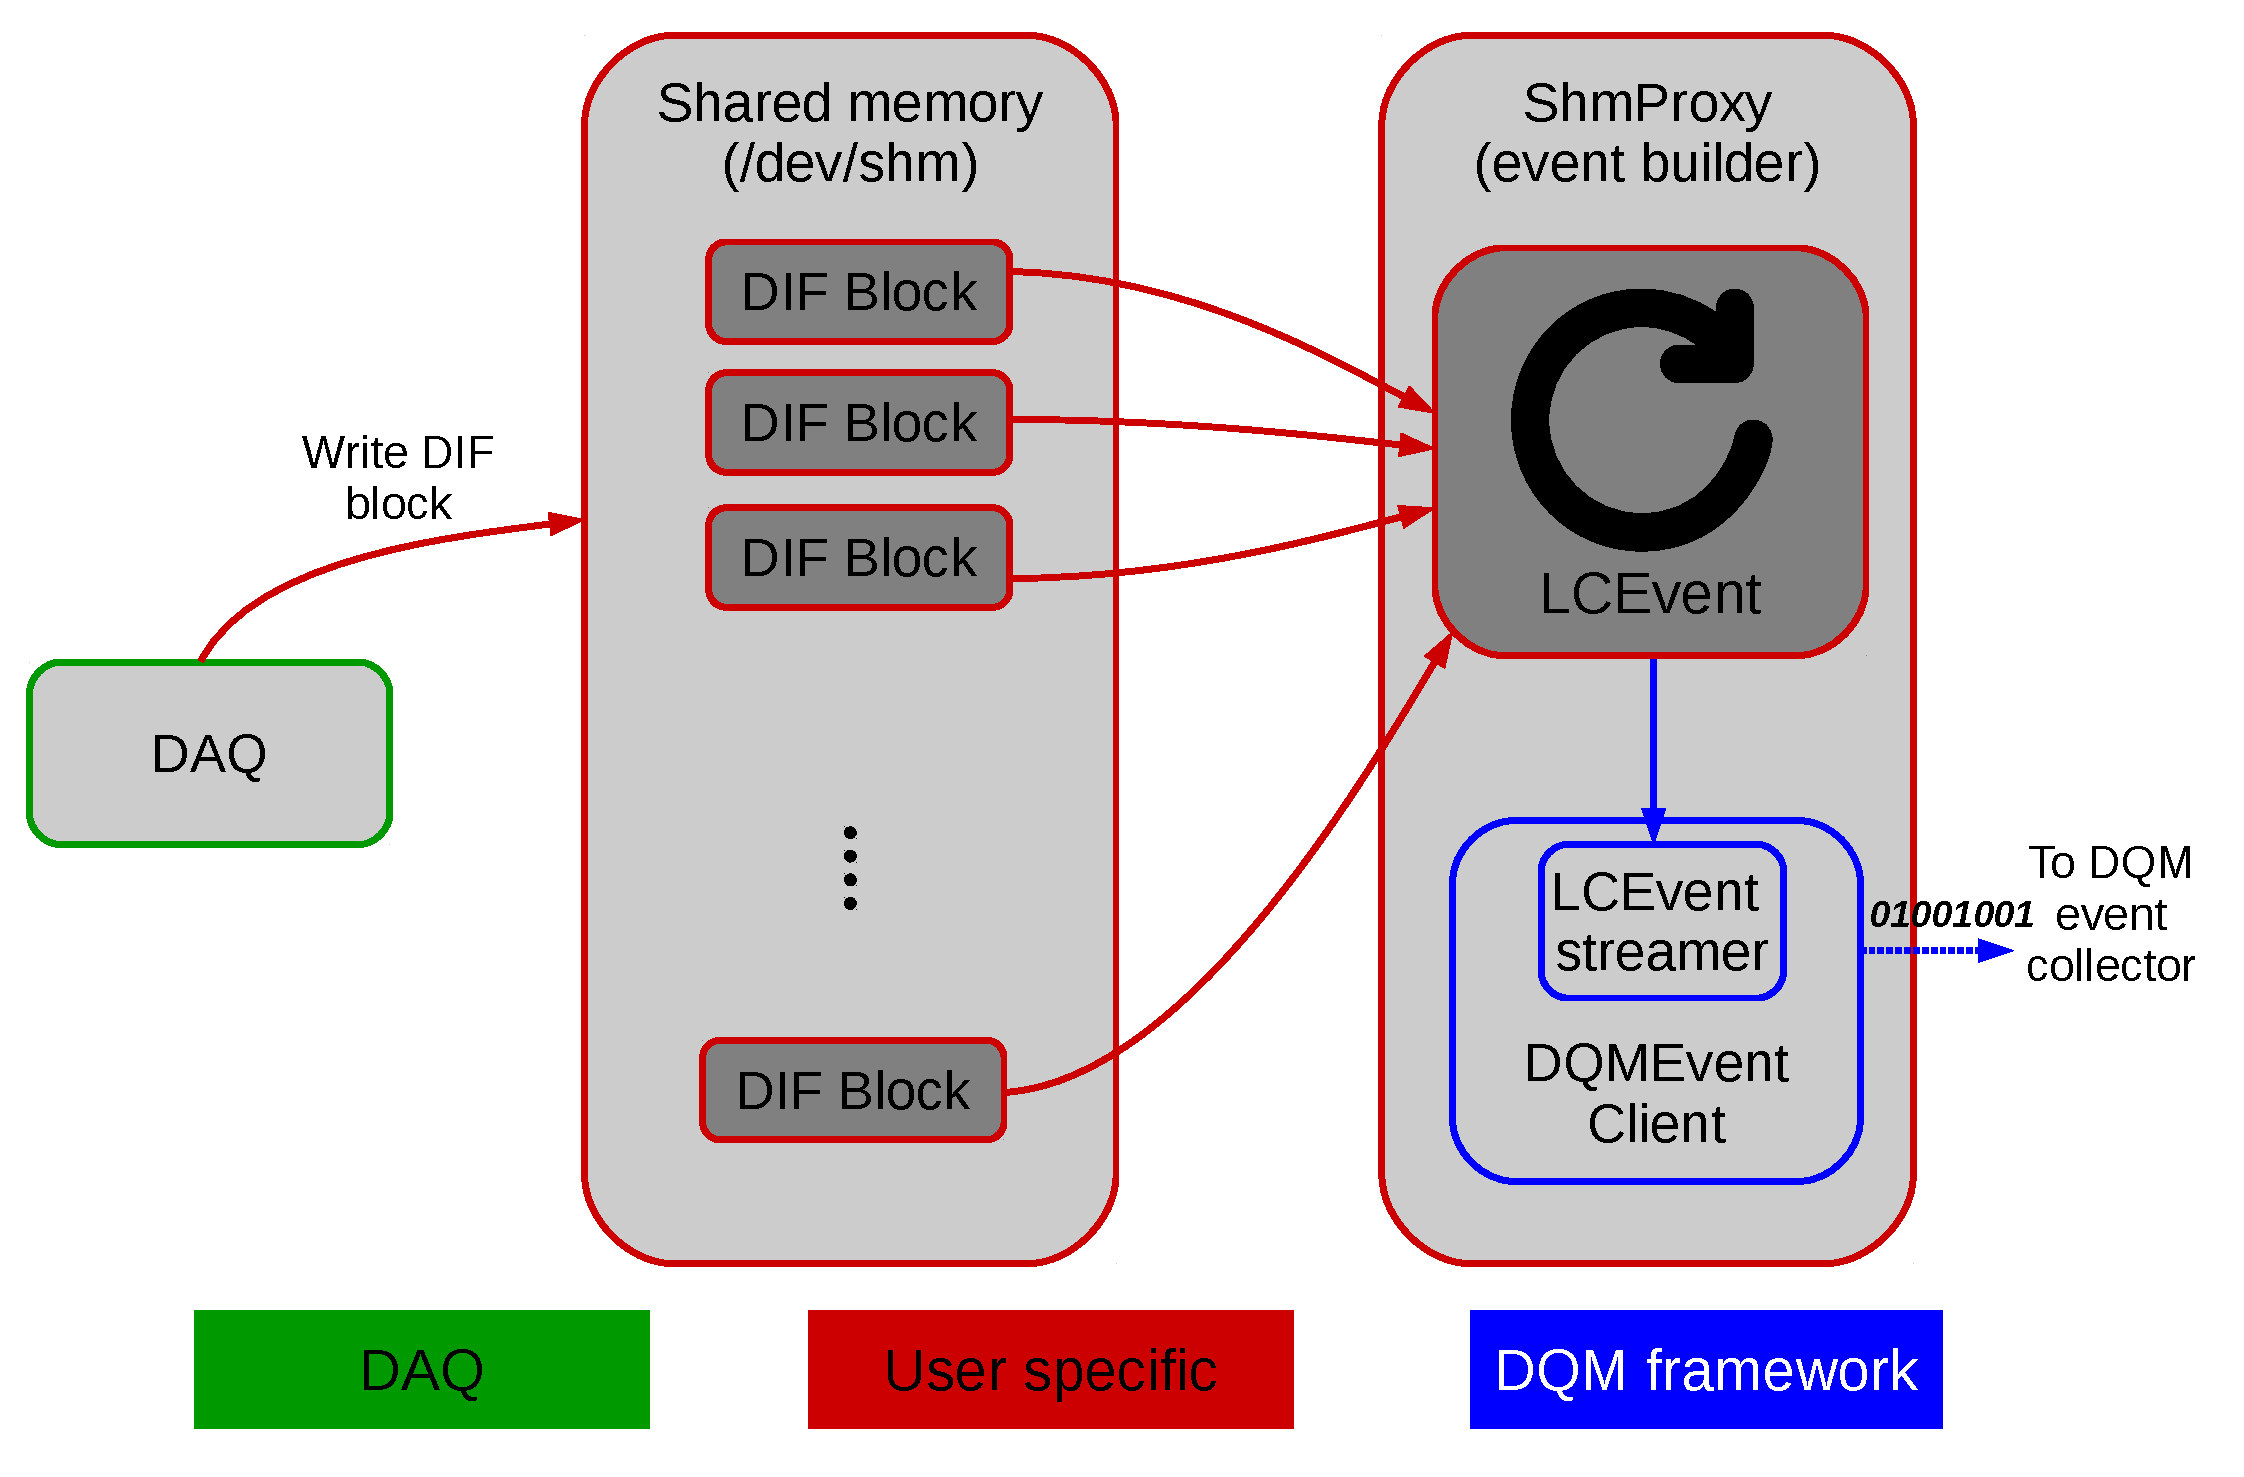
\includegraphics[width=0.9\textwidth]{figs/sdhcal_dqm_daq.pdf}
      \end{center}
    \end{frame}

  %% EVENT COLLECTORS %%
%   \begin{frame}[containsverbatim]
%     \frametitle{\secname}
%     \framesubtitle{Event collectors, client/server}
%
%     \begin{minipage}{0.52\textwidth}
%         Event collector (\verb|DQMEventCollector|) and \\
%         Event client (\verb|DQMEventClient|) \\
%         linked via DIM (TCP/IP).\\
%         ~ \\
%         Receiver interface with 2 modes :
%         \begin{itemize}
%           \item on update
%           \item on query
%         \end{itemize}
%         ~ \\
%         Sender interface with one unique command to send an event to the collector server \\
%         ~ \\
%         Use \verb|dqm4hep_start_event_collector| to start a collector server.
%     \end{minipage}
%     \begin{minipage}{0.42\textwidth}
%       \begin{center}
%         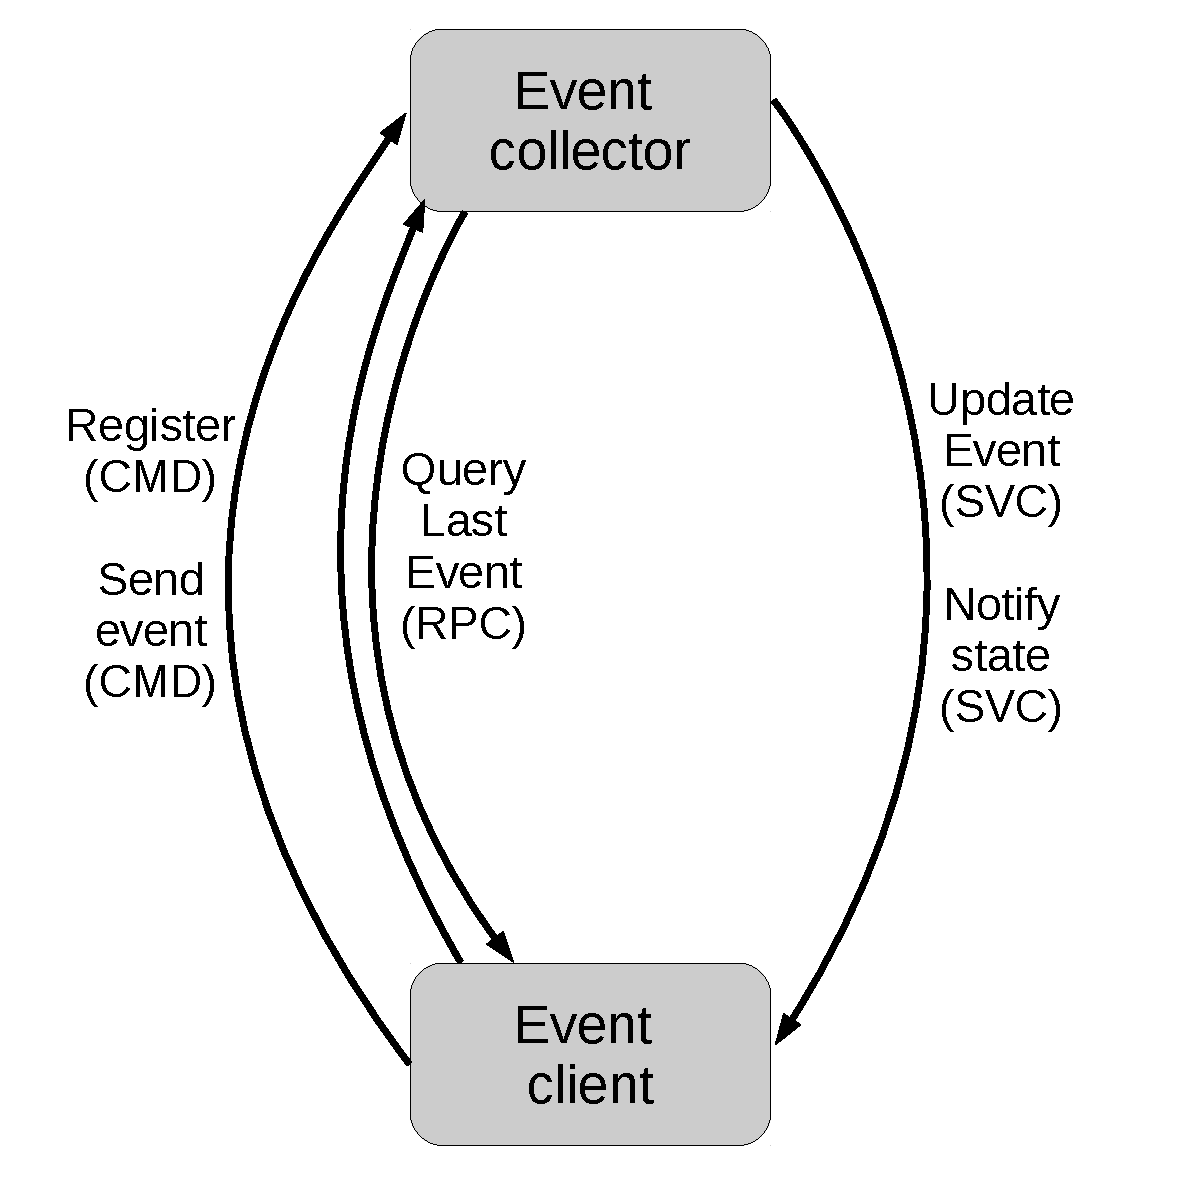
\includegraphics[width=\textwidth]{figs/event_collector_arch.pdf}
%       \end{center}
%     \end{minipage}
%
%   \end{frame}


  %% MODULE APPLICATION %%
  \begin{frame}[containsverbatim]
    \frametitle{\secname}
    \framesubtitle{Module applications - analysis module}

    \begin{minipage}{0.78\textwidth}
      \begin{block}{Purpose}
        \begin{itemize}
          \item Receive events from a collector server and process them
          \item Produce monitor elements (histograms, scalars, generic TObject)
          \item Follow the run control signals (SOR, EOR)
        \end{itemize}
      \end{block}

      \begin{itemize}
        \item \textbf{Init} : Initialize the application : load dlls, declare services, etc ... Wait for a SOR
        \item \textbf{Start of run} : start cycles loop, open archive
        \item \textbf{Start of cycle} : start a cycle of '\textit{process event}'
        \item \textbf{Process event} : Process incoming event, fill monitor elements, etc ...
        \item \textbf{End of cycle} : send subscribed monitor elements, update archive (opt).
        \item \textbf{End of run} : Wait for SOR, close archive (opt).
        \item \textbf{End} : Clean and exit module.
      \end{itemize}
      To implement online DQM analysis, user must implement the \verb|DQMAnalysisModule| interface. A shared library must be build and loaded in the application using the plugin system (\verb|export DQM4HEP_PLUGIN_DLL=libMyModule.so|). \\
      ~ \\
      Use \verb|dqm4hep_start_analysis_module| to start an analysis module.

    \end{minipage}
    \begin{minipage}{0.2\textwidth}
      \begin{flushright}
        \begin{tikzpicture}[scale=0.8]
        \node[draw] (I) at (0,-1) {Init};
        \node[draw] (SR) at (0,-2) {Start of run};
        \node[draw] (SC) at (0,-3) {Start of cycle};
        \node[draw] (PE) at (0,-4) {Process event};
        \node[draw] (EC) at (0,-5) {End of cycle};
        \node[draw] (ER) at (0,-6) {End of run};
        \node[draw] (E) at (0,-7) {End};
        \tikzset{fleche/.style={->,>=latex,thick}}
        \draw[fleche] (0,0) node {$\bullet$} -- (I);
        \draw[fleche] (I) -- (SR);
        \draw[fleche] (SR) -- (SC);
        \draw[fleche] (SC) -- (PE);
        \draw[fleche] (PE) -- (EC);
        \draw[fleche] (EC) -- (ER);
        \draw[fleche] (ER) -- (E);
        \draw[fleche] (E) -- (0,-8) node {$\bullet$};
        \draw[fleche] (0,-4.5) -- (1.3,-4.5) -- (1.3,-3.5) -- (0,-3.5);
        \draw[fleche] (0,-5.5) -- (1.4,-5.5) -- (1.4,-2.5) -- (0,-2.5);
        \draw[fleche] (0,-6.5) -- (1.5,-6.5) -- (1.5,-1.5) -- (0,-1.5);
        \end{tikzpicture}\\
        Analysis module~~~~\\ application flow~~~~~
      \end{flushright}
    \end{minipage}

  \end{frame}

  \begin{frame}
    \frametitle{\secname}
    \framesubtitle{Module API}
      \begin{center}
       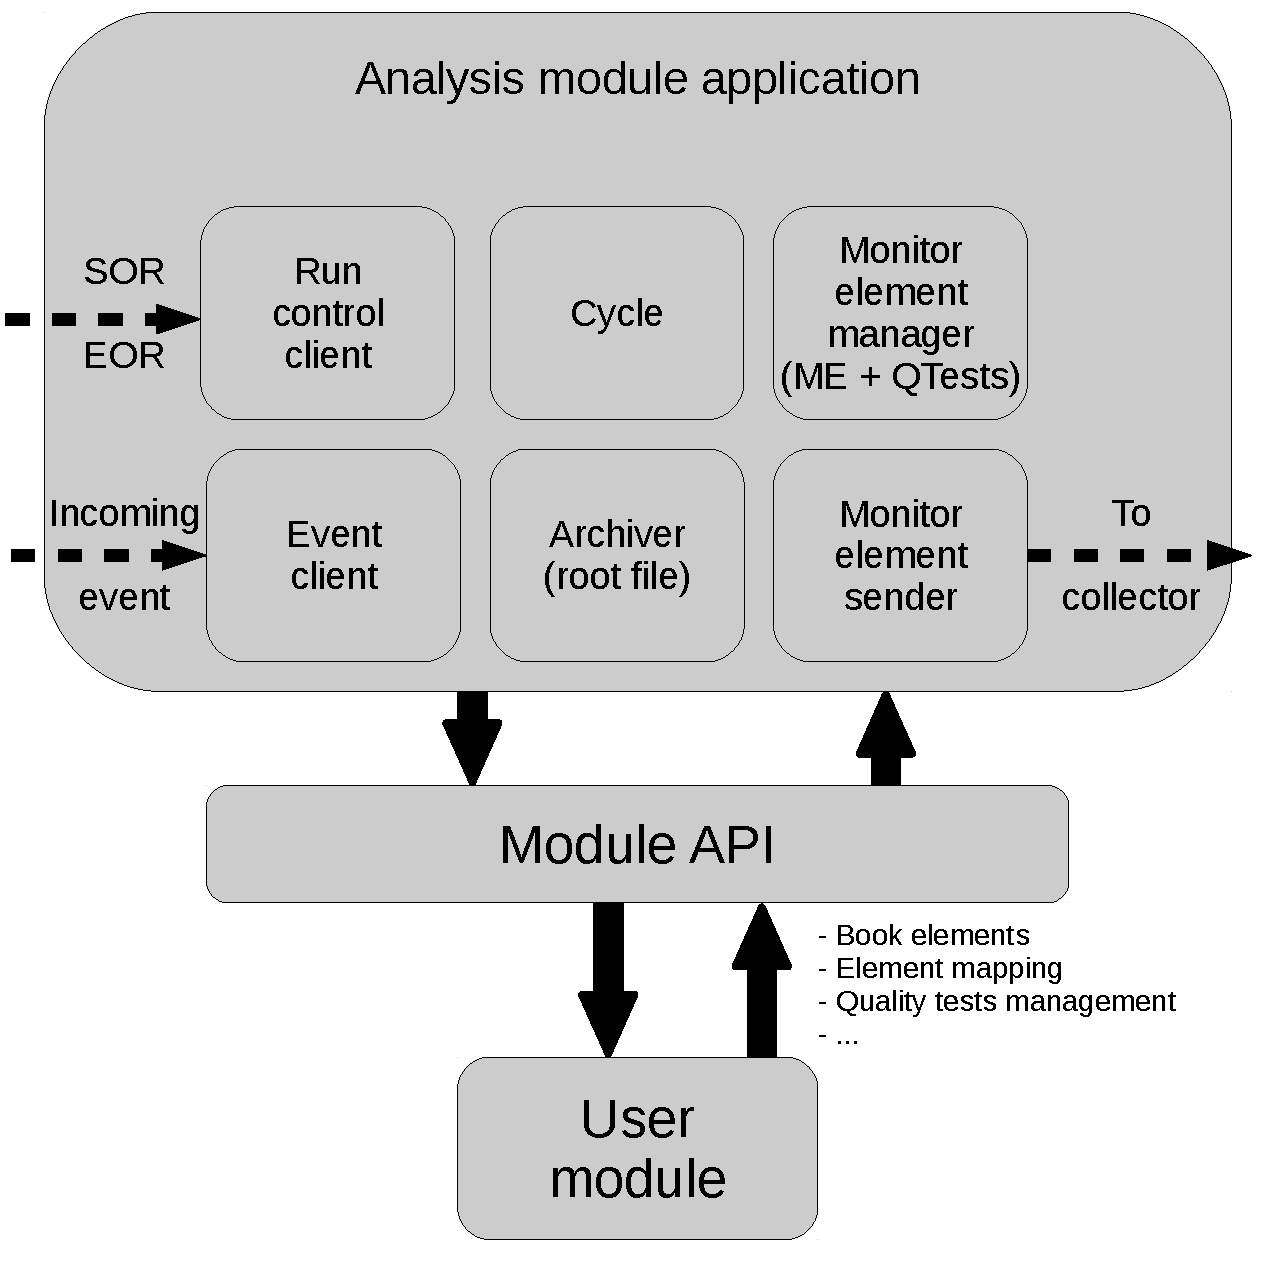
\includegraphics[width=0.6\textwidth]{figs/analysis_module_api.pdf}
      \end{center}
  \end{frame}


%   \begin{frame}[containsverbatim]
%     \frametitle{\secname}
%     \framesubtitle{Module applications - standalone module}
%
%     \begin{minipage}{0.78\textwidth}
%       \begin{block}{Purpose}
%         \begin{itemize}
%           \item No event reception
%           \item No run signals
%           \item Produce monitor elements (histograms, scalars, generic TObject)
%         \end{itemize}
%       \end{block}
%
%       \begin{itemize}
%         \item \textbf{Init} : Load dlls, init the module.
%         \item \textbf{Start of cycle} : start a timer cycle of n seconds
%         \item \textbf{Process} : call back function.
%         \item \textbf{End of cycle} : collect monitor elements and send
%         \item \textbf{End} : The application has received a signal to exit and the process ends.
%       \end{itemize}
%       To implement online standalone analysis, user must implement the \verb|DQMStandaloneModule| interface. A shared library must be build and loaded in the application using the plugin system (see next slides). \\
%       ~ \\
%       \textcolor{red}{Designed for \textit{slow control - like} data processing}. \\
%       ~ \\
%       Use \verb|dqm4hep_start_standalone_module| to start a standalone module.
%     \end{minipage}
%     \begin{minipage}{0.2\textwidth}
%       \begin{flushright}
%         \begin{tikzpicture}[scale=0.8]
%         \node[draw] (I) at (0,-1) {Init};
%         \node[draw] (SC) at (0,-2) {Start of cycle};
%         \node[draw] (PE) at (0,-3) {Process};
%         \node[draw] (EC) at (0,-4) {End of cycle};
%         \node[draw] (E) at (0,-5) {End};
%         \tikzset{fleche/.style={->,>=latex,thick}}
%         \draw[fleche] (0,0) node {$\bullet$} -- (I);
%         \draw[fleche] (I) -- (SC);
%         \draw[fleche] (SC) -- (PE);
%         \draw[fleche] (PE) -- (EC);
%         \draw[fleche] (EC) -- (E);
%         \draw[fleche] (E) -- (0,-6) node {$\bullet$};
%         \draw[fleche] (0,-3.5) -- (1.3,-3.5) -- (1.3,-2.5) -- (0,-2.5);
%         \draw[fleche] (0,-4.5) -- (1.4,-4.5) -- (1.4,-1.5) -- (0,-1.5);
%         \end{tikzpicture} \\
%         Standalone module~~~~\\ application flow~~~~~~~
%       \end{flushright}
%     \end{minipage}
%
%   \end{frame}

%   \begin{frame}
%     \frametitle{\secname}
%     \framesubtitle{Module API}
%       \begin{center}
%         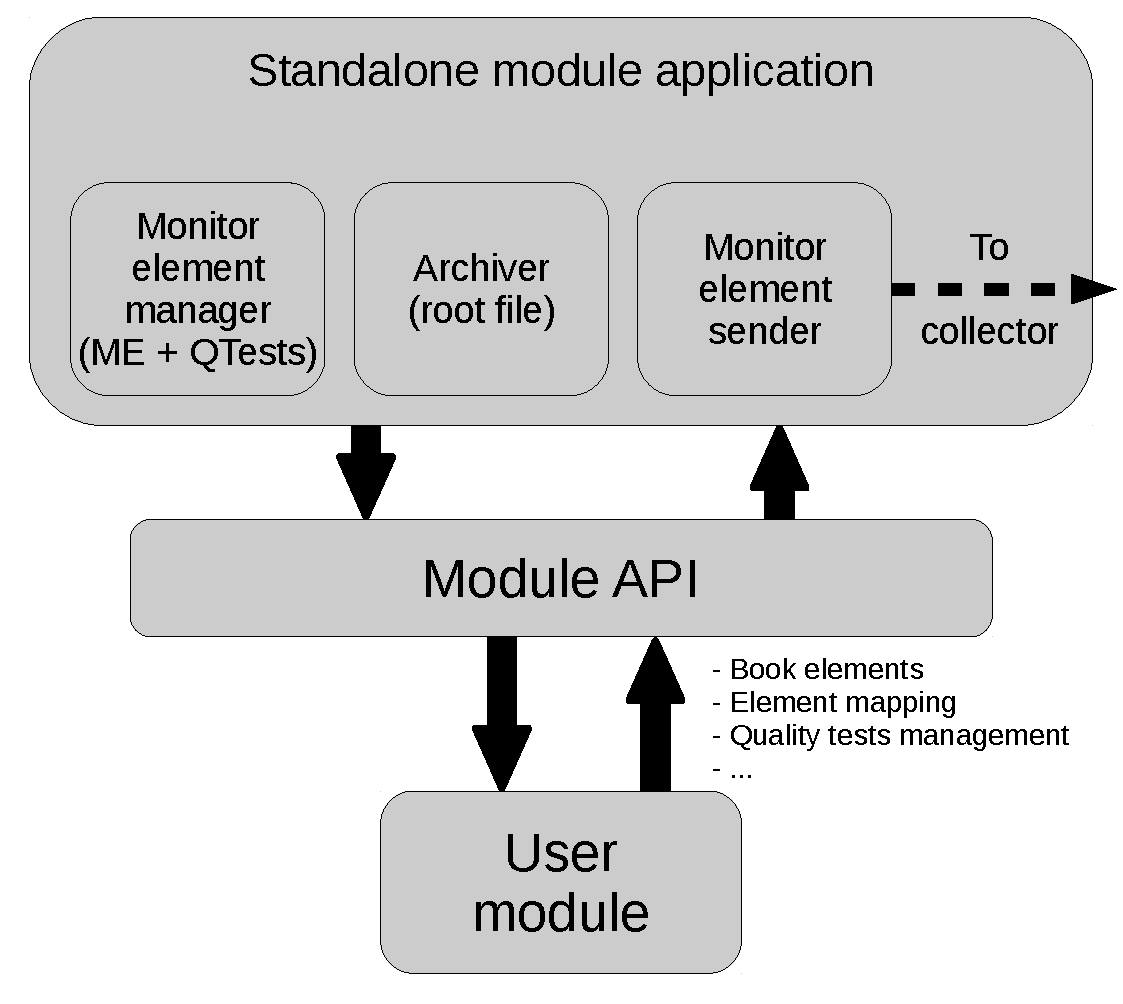
\includegraphics[width=0.6\textwidth]{figs/stand_module_api.pdf}
%       \end{center}
%   \end{frame}

  %% MONITOR ELEMENT COLLECTOR %%

%   \begin{frame}[containsverbatim]
%     \frametitle{\secname}
%     \framesubtitle{Monitor element collector, client/server}
%
%     \begin{minipage}{0.43\textwidth}
%       Collect monitor elements from different modules. \\
%       ~ \\
%       Publish/subscribe paradigm with client side. \\
%       ~ \\
%       Collector stores the available list of elements (names) from the different modules and the elements that the clients have subscribed.
%     \end{minipage}
%     \begin{minipage}{0.55\textwidth}
%       \begin{center}
%         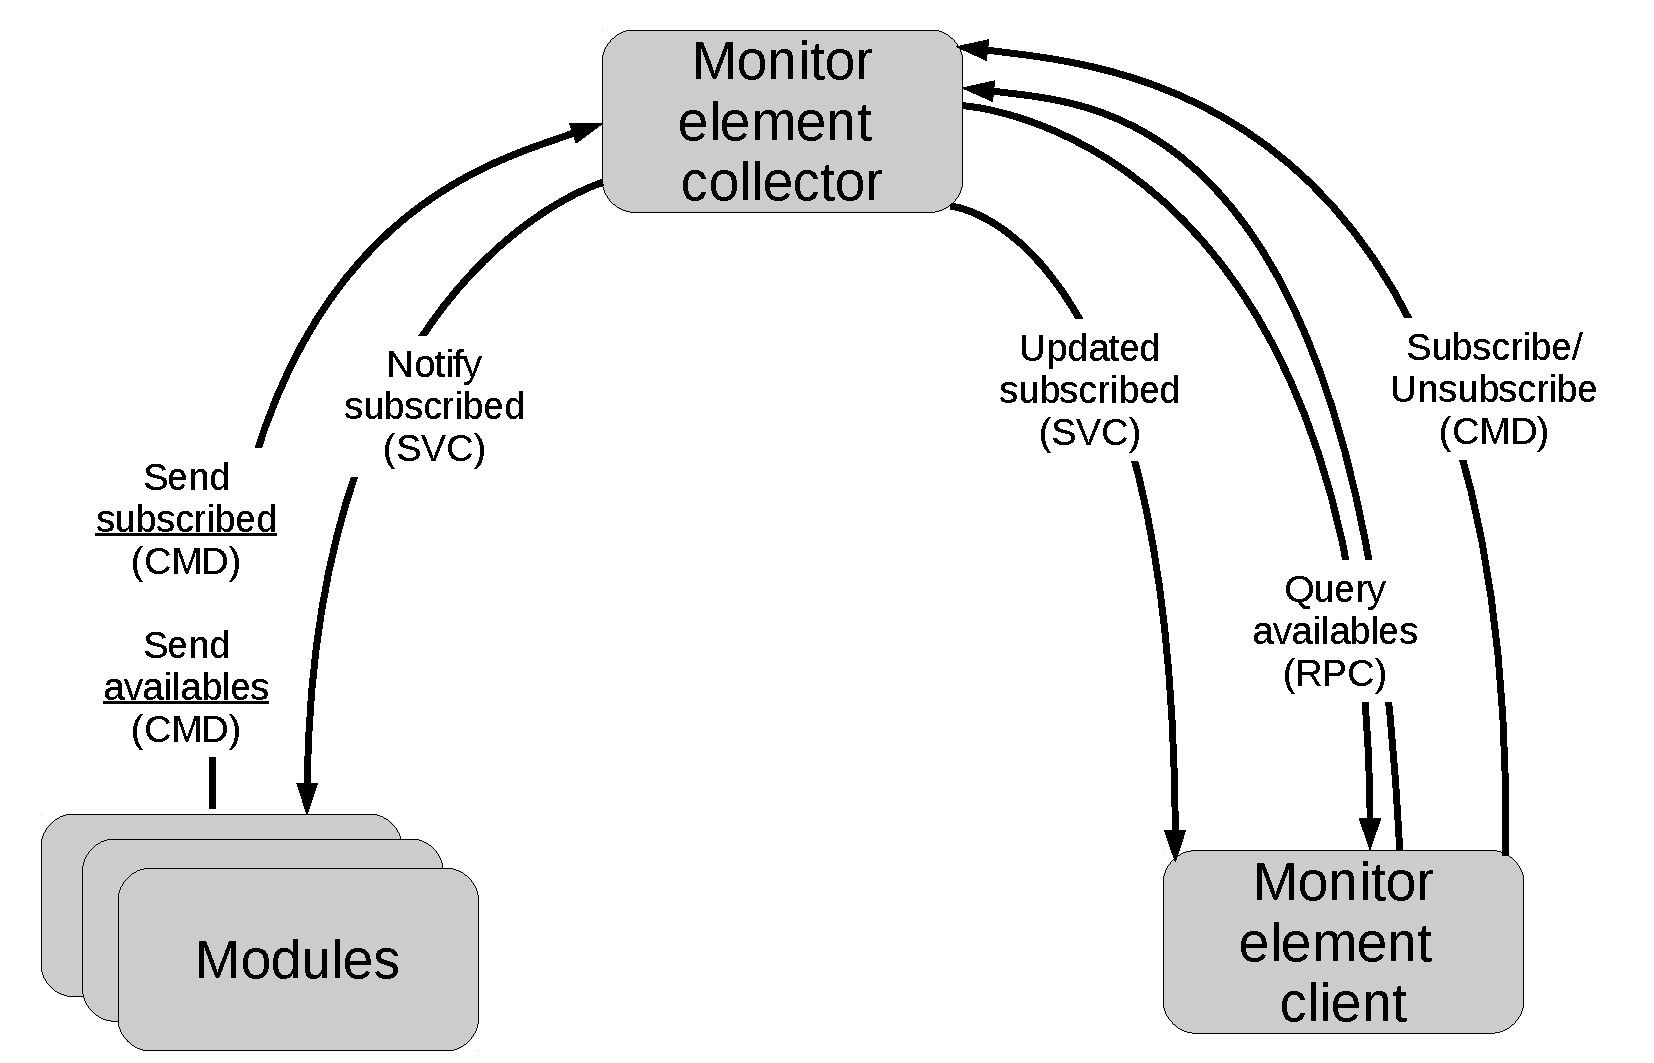
\includegraphics[width=\textwidth]{figs/me_collector_arch.pdf}
%       \end{center}
%     \end{minipage}
%     ~ 
%     ~ \\
%     Client interface works on both update and query modes. \\
%     ~ \\
%     Use \verb|dqm4hep_start_monitor_element_collector| monitor element collector.
%
%   \end{frame}




    %% USER INTERFACE OVERVIEW %%
%     \section{User interfaces overview}
%
%     \begin{frame}[containsverbatim]
%       \frametitle{\secname}
%       \framesubtitle{Plugin system}
%
%       The core part of the system provides a plugin system, massively used by the framework to handle user classes. \\
%       ~ \\
%       The \verb|DQMPluginManager| singleton class manages the plug-ins provided by the system and the users. Plugins can be loaded at any time by loading shared libraries. \\
%       ~ \\
%       Example :
%       \begin{lstlisting}
%       // single library loading
%       DQMPluginManager::instance()->loadLibrary("libMyClass.so");
%       // multiple libraries loading
%       StringVector libraries = { "libMyClass.so" , "libAnotherClass.so" }
%       DQMPluginManager::instance()->loadLibraries(libraries);
%       // using DQM4HEP_PLUGIN_DLL env var with ':' separation
%       // assuming export DQM4HEP_PLUGIN_DLL=./lib/libSuperClass.so:./lib/libDirtyClass.so
%       DQMPluginManager::instance()->loadLibraries();
%       \end{lstlisting}
%
%       ~ \\
%       In principle \textbf{any} user class can be plugged in the framework and retrieved inside applications. \\
%       ~ \\
%     \end{frame}


%     \begin{frame}[containsverbatim]
%       \frametitle{\secname}
%       \framesubtitle{Plugin system}
%       User Example :
%       \begin{lstlisting}
%       // MyClass.h
%       class MyClass
%       {
%         public:
%           MyClass(); // Default constructor mandatory !!
%         private:
%           int    m_attribute;
%       };
%       // MyClass.cc
%       DQM_PLUGIN_DECL( MyClass , "MyClass" ) // plug the class in the system
%
%       MyClass::MyClass() : m_attribute(0) {}
%       // ...
%       \end{lstlisting}
%       %\pause
%
%       To get an instance of your class, use the plugin manager :
%       \begin{lstlisting}
%       // ...
%       MyClass *pClass = DQMPluginManager::instance()->createPluginClass<MyClass>("MyClass");
%       // ...
%       \end{lstlisting}
%
%       For example, this functionality is used internally to get :
%       \begin{itemize}
%         \item user module implementations
%         \item event streamers
%         \item run control clients
%       \end{itemize}
%
%     \end{frame}




    %% STREAMER INTERFACE %%
%     \begin{frame}[containsverbatim]
%     \frametitle{\secname}
%     \framesubtitle{Streaming interface}
%
%       \textbf{The framework has \textcolor{red}{no dependency on the type of data} transferred over the network!} \\
%       ~ \\
%       For example, the streamer for LCIO is implemented and provided as a plug-in in the software. The type of data that is transferred over the network can be user defined. \\
%       Users have to implements the \verb|DQMEventStreamer| interface : \\
%
%       \begin{lstlisting}
%       class DQMEventStreamer : public DQMStreamer<DQMEvent>
%       {
%       public:
%         // ...
%         virtual StatusCode serialize(const DQMEvent *const pEvent, DQMDataStream *const pDataStream) = 0;
%         virtual StatusCode deserialize(DQMEvent *&pEvent, DQMDataStream *const pDataStream) = 0;
%         virtual StatusCode serialize(const DQMEvent *const pEvent, const std::string &subEventIdentifier, DQMDataStream *const pDataStream) = 0;
%       };
%       \end{lstlisting}
%
%       and plug the streamer class using the plugin mechanism. The \verb|DQMDataStream| class provides functions to read and write raw buffers. \\
%       ~ \\
%       For an experiment with a simple event structure, it can be useful to define a raw event streamer and propagate the event through the DQM system without taking care about the network interface. \\
%     \end{frame}







    %% MODULE API %%
    \begin{frame}[containsverbatim]
      \frametitle{\secname}
      \framesubtitle{Module API}

      \begin{block}{Monitor element management}
        \begin{itemize}
          \item Memory management
          \item Booking methods (book, delete, from xml)
          \item Access management via an internal map ("name" -> element)
          \item Directory management : mkdir, cd, ls, rmdir, pwd
        \end{itemize}
      \end{block}

      \begin{block}{Quality tests}
        Quality tests used to \textbf{evaluate the quality} of a particular monitor element. \\
        Example of quality tests :
        \begin{itemize}
          \item Kolmogorov test with a reference histogram
          \item $\chi^2$ test after a histogram fit
        \end{itemize}
        Quality tests can also be \textbf{user defined} (via \verb|DQMQualityTestFactory| class). \\
        Quality tests results (\verb|DQMQualityTestResult| class) stored within monitor element and both \textbf{sent to the collector}. \\
        The module API provides functions for :
        \begin{itemize}
          \item User QTests registration
          \item QTests assignment to monitor elements (also from xml)
          \item QTest results access (read only)
        \end{itemize}
      \end{block}
    \end{frame}


    %% MODULE EXAMPLE %%
    \begin{frame}[containsverbatim]
      \frametitle{\secname}
      \framesubtitle{Analysis module - Example }

      \begin{minipage}{0.49\textwidth}
        \begin{lstlisting}
// ExampleModule.h
class ExampleModule : public DQMAnalysisModule
{
public:
  ExampleModule();  // requiered by plugin system
  ~ExampleModule();

  StatusCode initModule();
  StatusCode readSettings(const TiXmlHandle &xmlHandle);
  StatusCode startOfRun(DQMRun *const pRun);
  StatusCode startOfCycle();
  StatusCode processEvent(DQMEvent *const pEvent);
  StatusCode endOfCycle();
  StatusCode endOfRun(DQMRun *const pRun);
  StatusCode endModule();

private:
  DQMMonitorElement   *m_pNHitElement;
};
        \end{lstlisting}
      \end{minipage}
      \begin{minipage}{0.49\textwidth}
        \begin{lstlisting}
// ExampleModule.cc
#include "ExampleModule.h"
// declare plugin in the system
DQM_PLUGIN_DECL( ExampleModule, "ExampleModule" )
// create and enter dir. Book histogram
StatusCode ExampleModule::initModule()
{
  DQMModuleApi::mkdir(this, "/Histograms");
  DQMModuleApi::cd(this, "/Histograms");
  DQMModuleApi::bookIntHistogram1D(this, m_pNHitElement, "NHit",
    "Number of hits", 1200, 0, 1199);
  return STATUS_CODE_SUCCESS;
}
// get lcio event and fill your histogram !
StatusCode ExampleModule::processEvent(DQMEvent *const pEvent)
{
  EVENT::LCEvent *pLCEvent =
    pEvent->getEvent<EVENT::LCEvent>();
  if(!pLCEvent)
    return STATUS_CODE_FAILURE;
    // get number of hits from a collection
  m_pNHitElement->get<TH1I>()->Fill(NHit);
  return STATUS_CODE_SUCCESS;
}
        \end{lstlisting}
      \end{minipage}


    \end{frame}











  \begin{frame}
    \frametitle{\secname}
    \framesubtitle{Gui visualisation}

	  Gui interfaces for DQM client developed :

      \begin{itemize}
        \item Run control, job control, online monitoring
        \item Written with Qt4 framework     
\includegraphics[width=.03\textwidth]{logo/Qt_CMYK_color}
        \item Easily configurable with json and xml.
      \end{itemize}

      \end{frame}


 %% Run Control %%
 \begin{frame}
    \frametitle{\secname}
    \framesubtitle{ Run Control GUI }
    \begin{center}
      \begin{overlayarea}{\textwidth}{\textheight}
      \begin{columns}
    	\column{.3\textwidth}
	           \vspace{-2em}
           \begin{center}
          \begin{onlyenv}<1>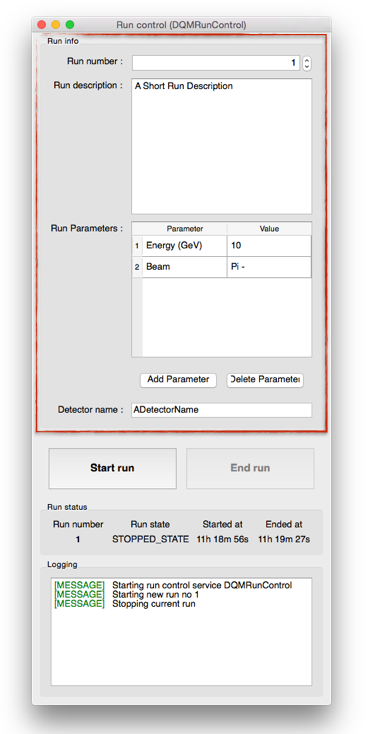
\includegraphics[width=\textwidth]{figs/RunControl/RunControl_Infos.png}\end{onlyenv}
          \begin{onlyenv}<2>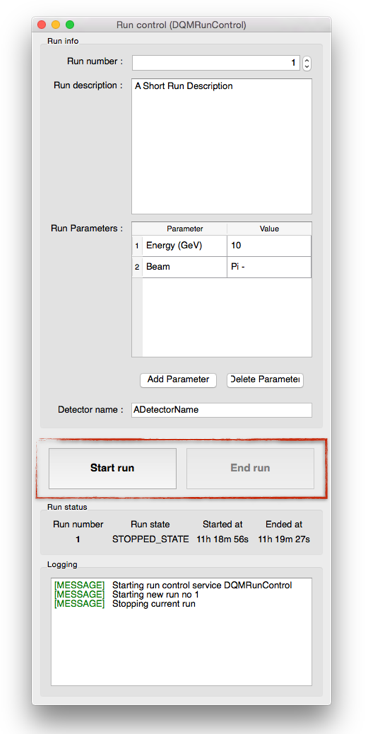
\includegraphics[width=\textwidth]{figs/RunControl/RunControl_SOR.png}\end{onlyenv}
          \begin{onlyenv}<3>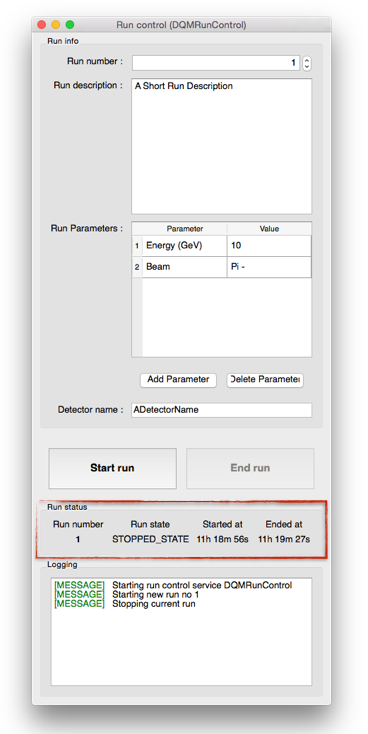
\includegraphics[width=\textwidth]{figs/RunControl/RunControl_Status.png}\end{onlyenv}
          \begin{onlyenv}<4>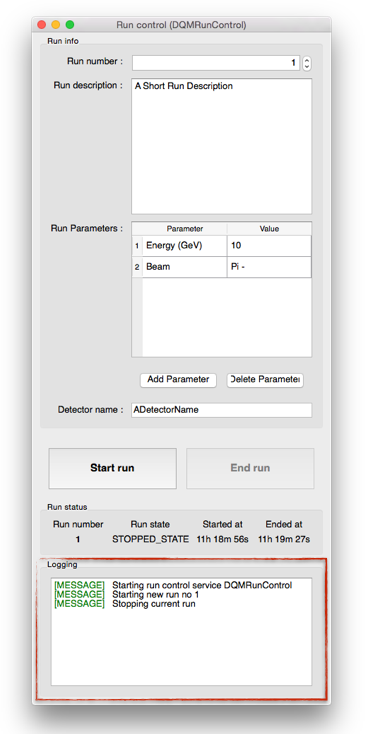
\includegraphics[width=\textwidth]{figs/RunControl/RunControl_logging.png}\end{onlyenv}
        \end{center}
    	\column{.7\textwidth}
        \begin{itemize}
         \uncover<1->{ \item Parametrisation of run with run number, detector name, run description and parameters }
       	 \uncover<2->{ \item Send SOR and EOR signals }
       	 \uncover<3->{\item Control run status ( State, Started/Stopped time ) }
       	 \uncover<4->{\item Every action is logged for easy information overview }
      \end{itemize}

      \end{columns}
      \end{overlayarea}
    \end{center}
  \end{frame}


 %% Job Interface %%
  \begin{frame}
    \frametitle{\secname}
    \framesubtitle{ Job Control GUI }

      \begin{overlayarea}{\textwidth}{\textheight}
      	\begin{center}
        		\begin{onlyenv}<5>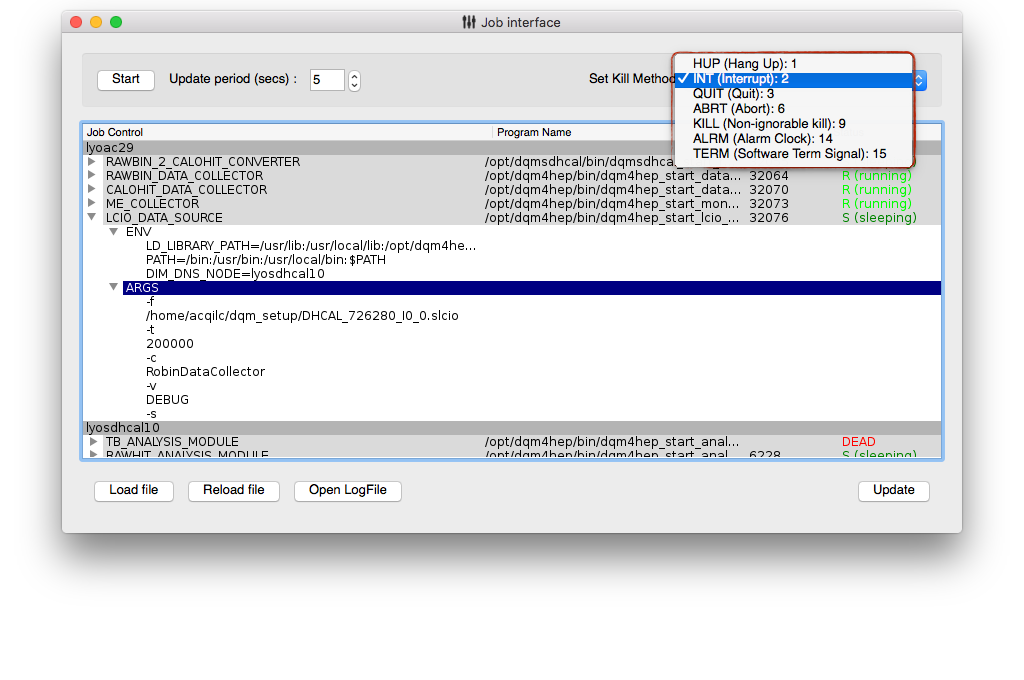
\includegraphics[width=0.8\textwidth]{figs/JobInterface/JobInterface_KillSwitch.png}\end{onlyenv}
       		\begin{onlyenv}<2>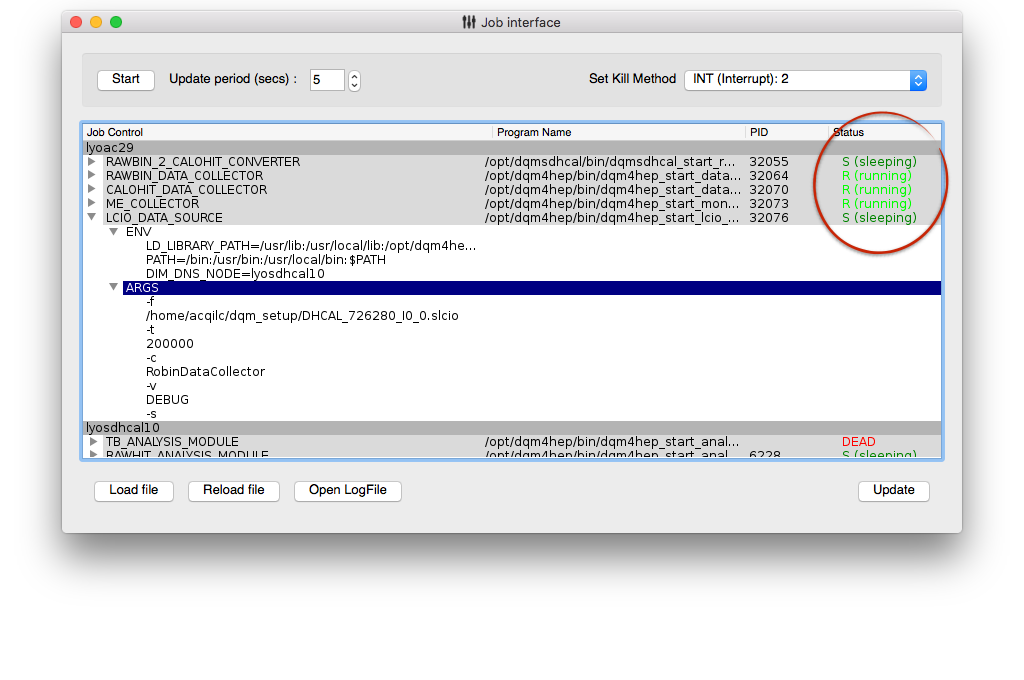
\includegraphics[width=0.8\textwidth]{figs/JobInterface/JobInterface_LiveStatus.png}\end{onlyenv}
        		\begin{onlyenv}<4>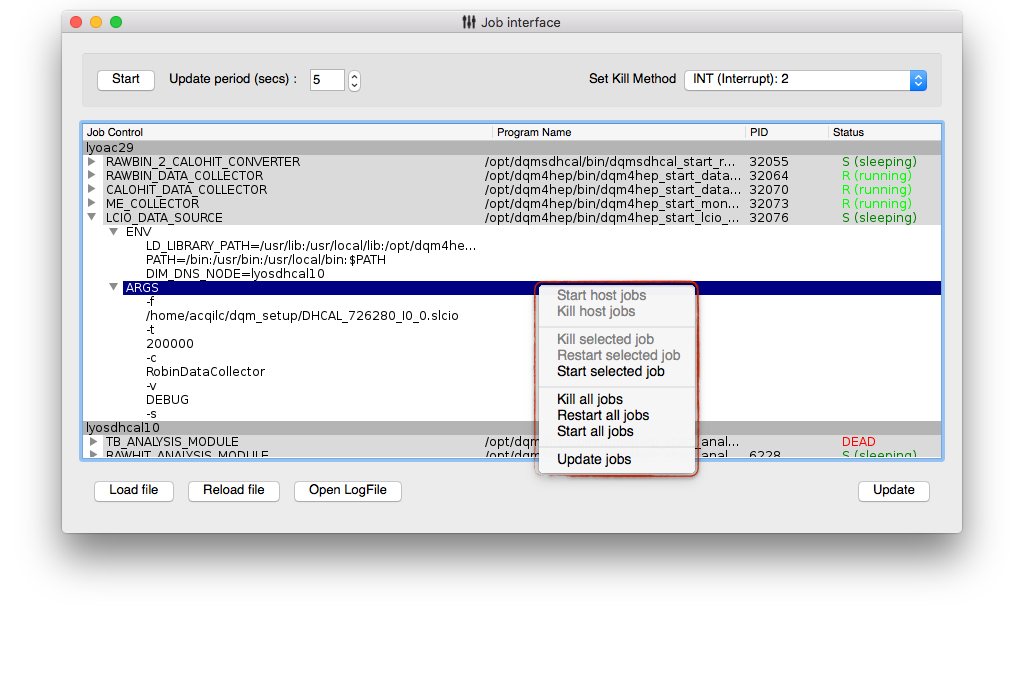
\includegraphics[width=0.8\textwidth]{figs/JobInterface/JobInterface_Module.png}\end{onlyenv}
        		\begin{onlyenv}<1>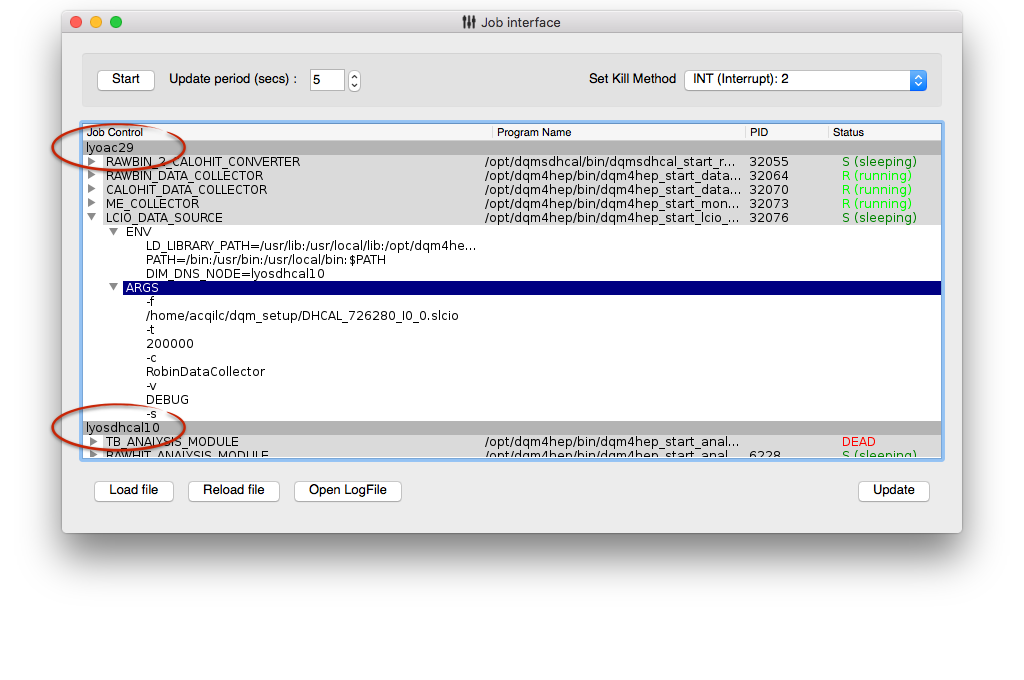
\includegraphics[width=0.8\textwidth]{figs/JobInterface/JobInterface_MultiHost.png}\end{onlyenv}
        		\begin{onlyenv}<3>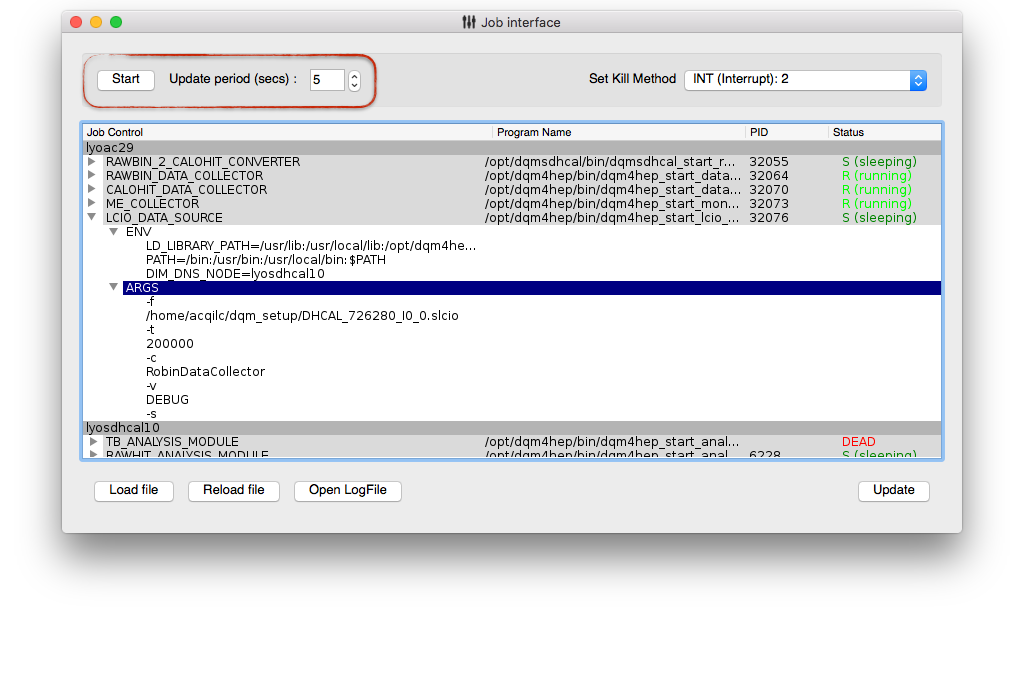
\includegraphics[width=0.8\textwidth]{figs/JobInterface/JobInterface_Update.png}\end{onlyenv}
      \end{center}
      \vspace{-5em}
       \begin{minipage}{\textwidth}

        \begin{itemize}
         \uncover<1->{ \item Load and display a list of applications (Collectors, Modules, etc.) available on different hosts }
       	 \uncover<2->{ \item Displays informations(Name, Host, PID, Status, etc.) about applications }
	 \uncover<3->{ \item Infos can be updated in "real time"}
       	 \uncover<4->{\item Manage Applications (Start/Kill/Restart) with contextual menu }
       	 \uncover<5->{\item Kill method can be adjusted }
      \end{itemize}

    \end{minipage}


    \end{overlayarea}
  \end{frame}


   %% Monitoring Control %%
   %% Browser %%
 \begin{frame}
    \frametitle{\secname}
    \framesubtitle{ Monitoring Gui + Browser }

    \begin{overlayarea}{\textwidth}{\textheight}
    	       \begin{center}

        \begin{onlyenv}<1>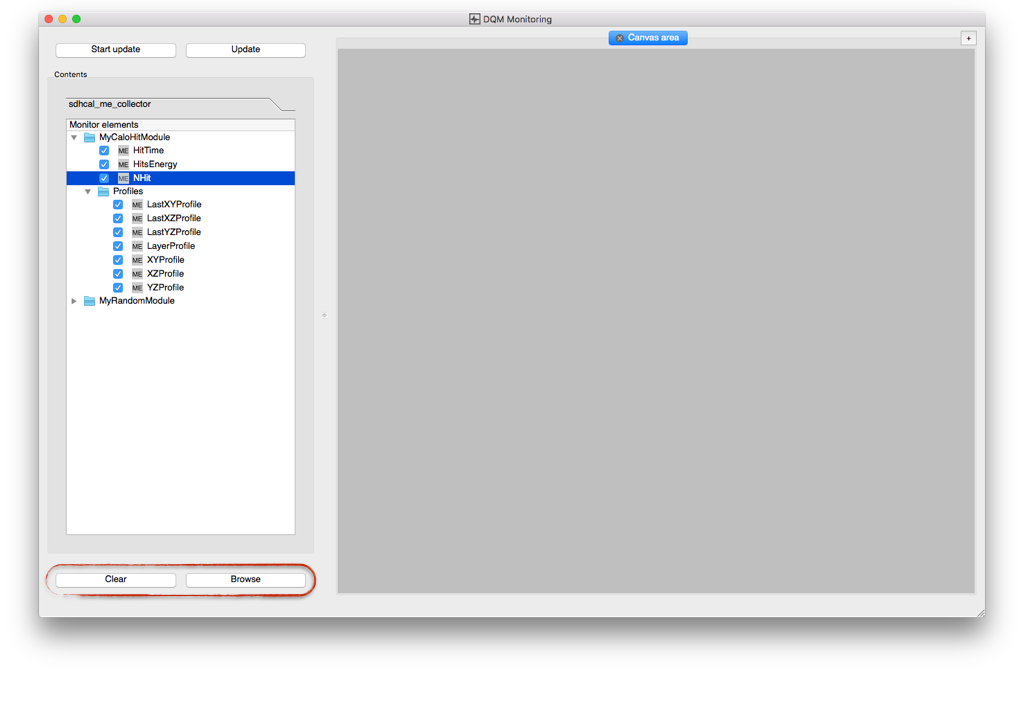
\includegraphics[width=0.8\textwidth]{figs/MonitoringGui/MG_Browse.png}\end{onlyenv}
                       \end{center}

       \begin{columns}

	 \column{.55\textwidth}
	 \vspace{-3em}

	\begin{center}
%          \begin{onlyenv}<2>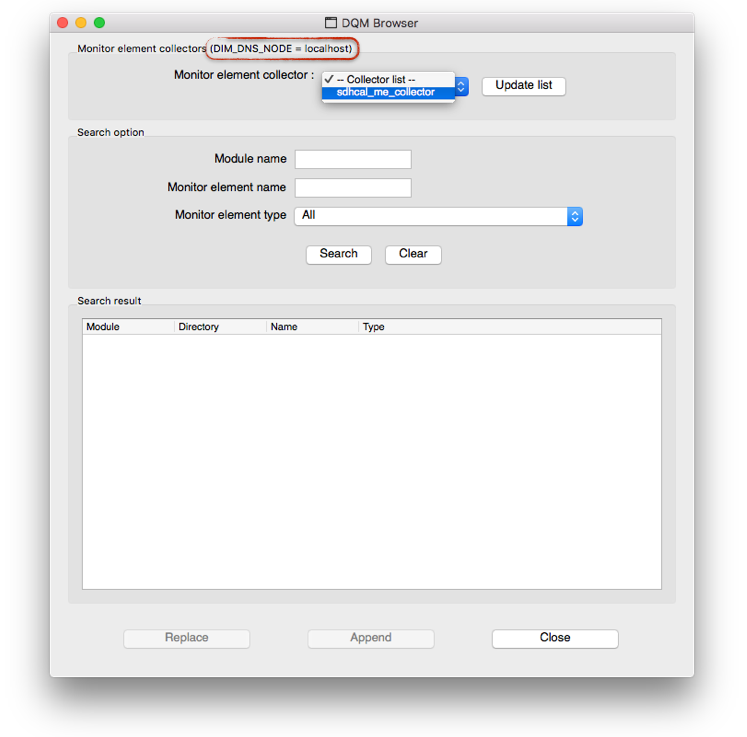
\includegraphics[width=1.1\textwidth]{figs/Browser/Browser_DNSNode.png}\end{onlyenv}
%          \begin{onlyenv}<3>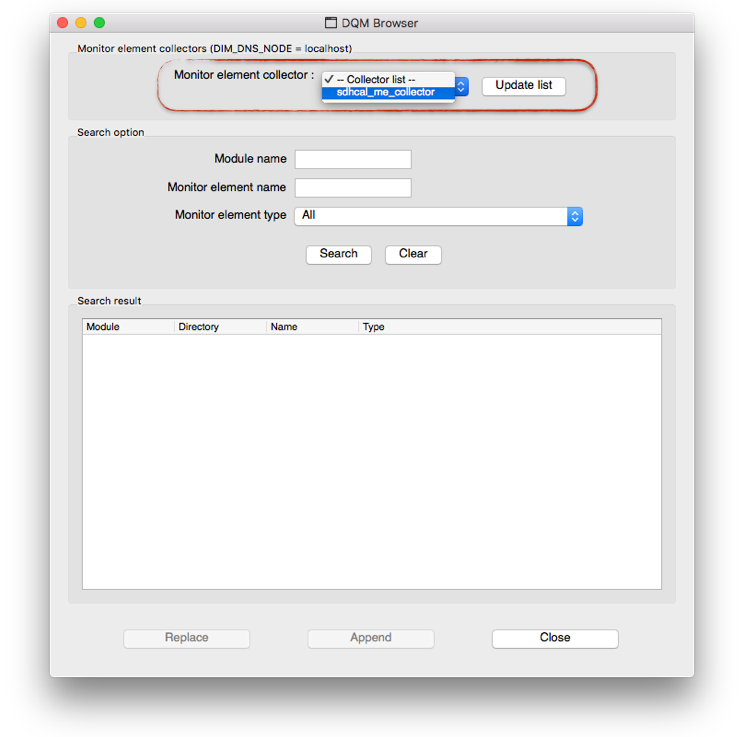
\includegraphics[width=1.1\textwidth]{figs/Browser/Browser_MESelection}\end{onlyenv}
%          \begin{onlyenv}<4>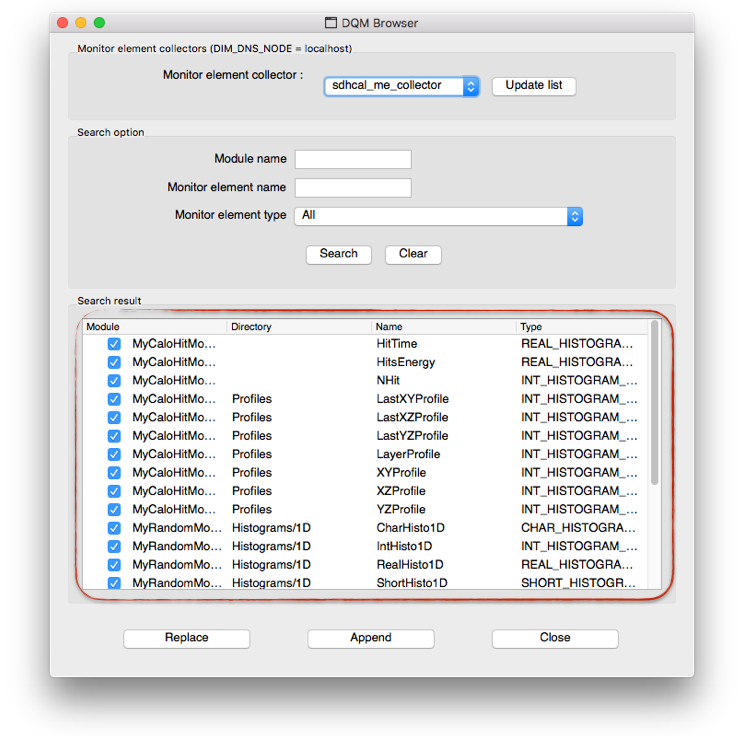
\includegraphics[width=1.1\textwidth]{figs/Browser/Browser_FullList}\end{onlyenv}
%          \begin{onlyenv}<5>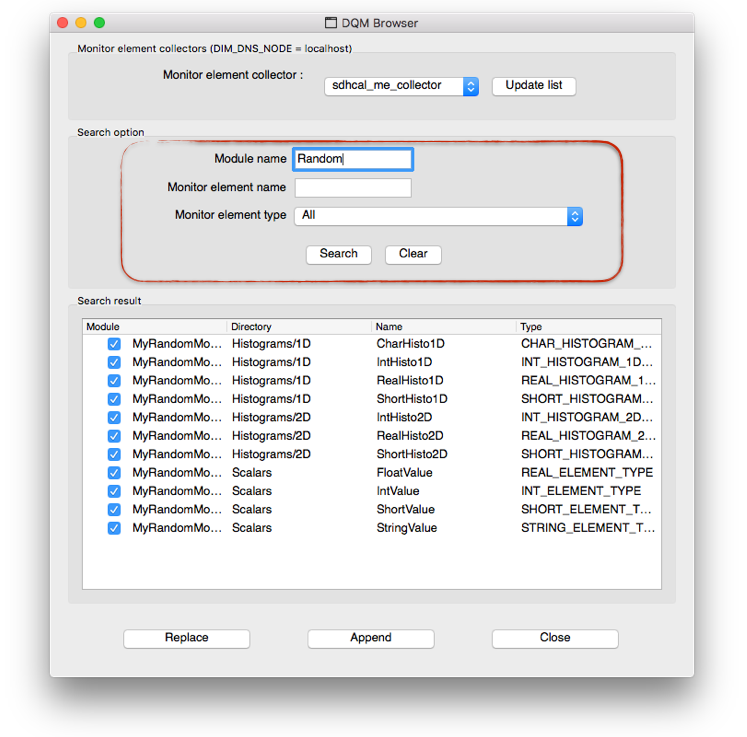
\includegraphics[width=1.1\textwidth]{figs/Browser/Browser_Search}\end{onlyenv}
         \begin{onlyenv}<2>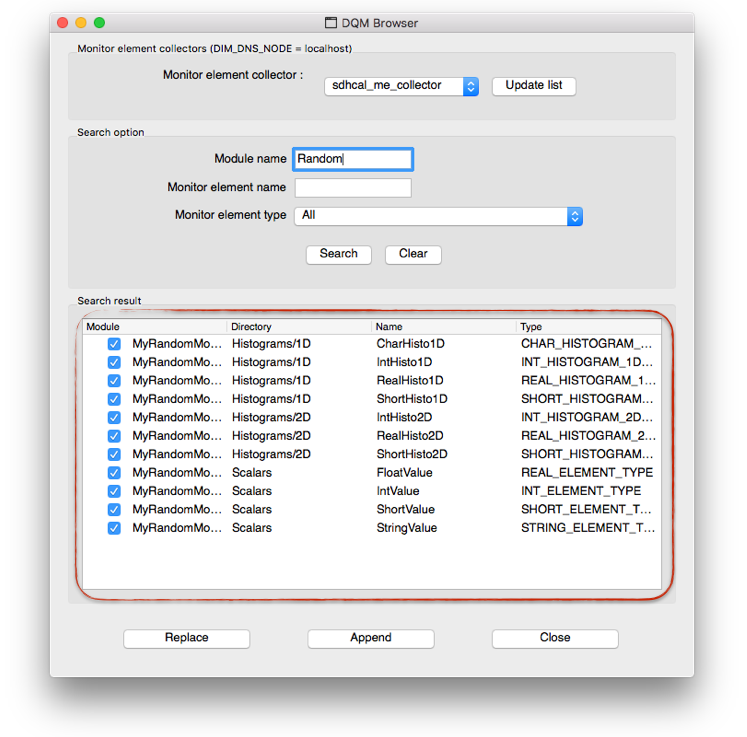
\includegraphics[width=1.1\textwidth]{figs/Browser/Browser_SearchResult}\end{onlyenv}
               \end{center}

         \column{.45\textwidth}
         \begin{itemize}
         \uncover<2->{ \item Browser to build histograms selections to display }
       	 \uncover<2->{\item Search Function to refine selection }
      \end{itemize}

           \end{columns}
               \end{overlayarea}

  \end{frame}


 %% Control Gui %%
\begin{frame}
    \frametitle{\secname}
    \framesubtitle{ Monitoring Gui + Browser }

        \begin{overlayarea}{\textwidth}{\textheight}
\vspace {-1em}
      \begin{center}

         \begin{onlyenv}<1>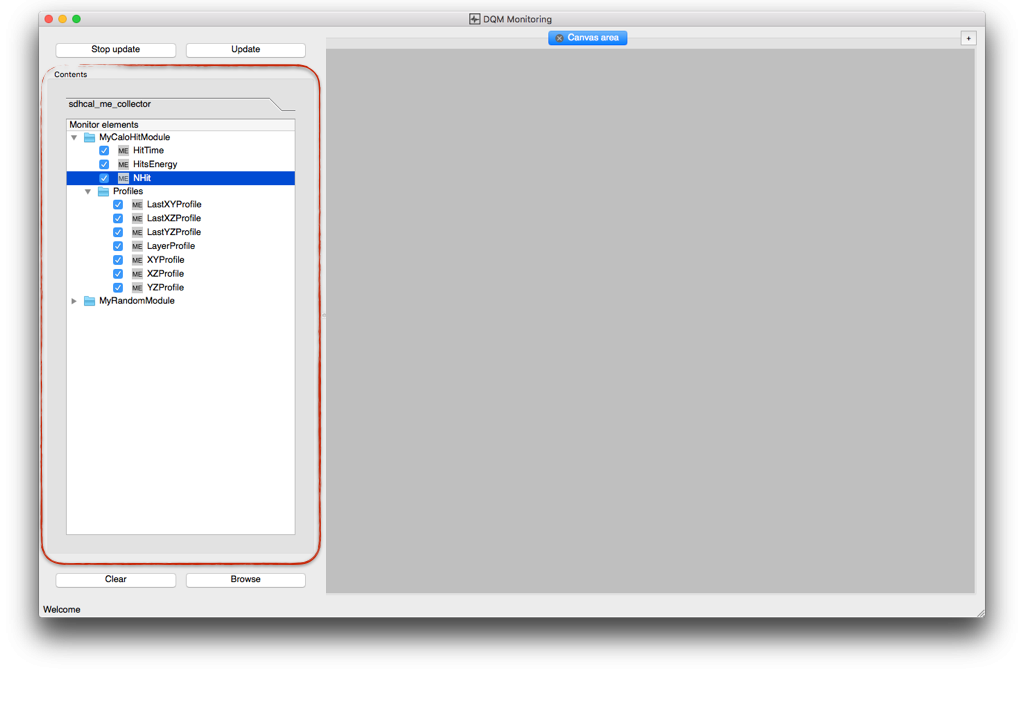
\includegraphics[width=0.8\textwidth]{figs/MonitoringGui/MG_Content}\end{onlyenv}
         \begin{onlyenv}<2>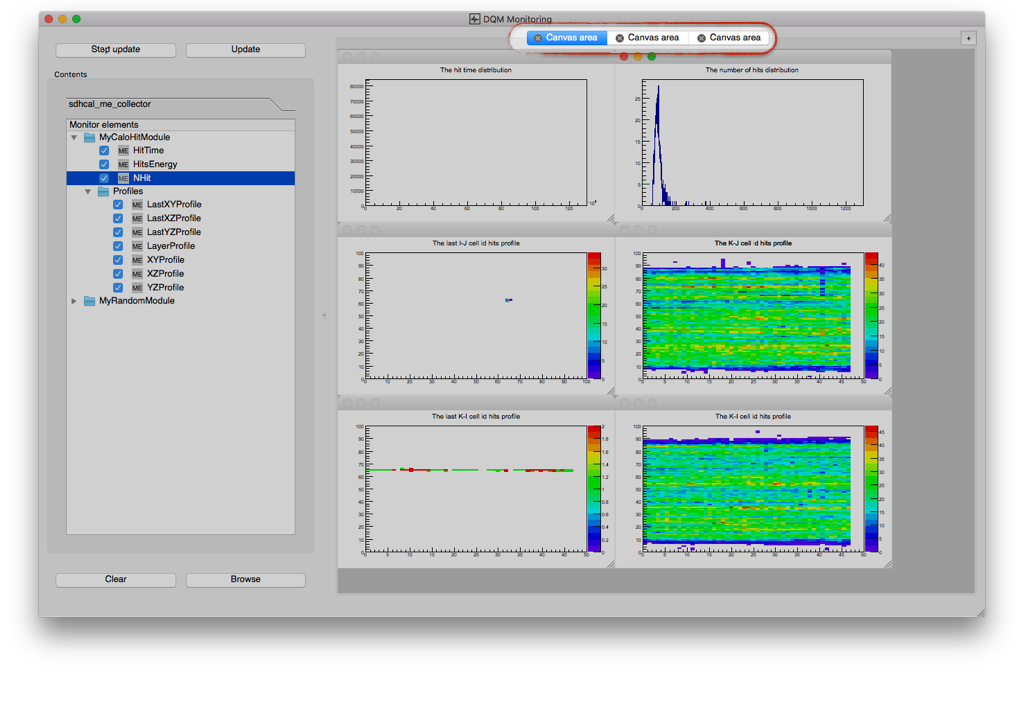
\includegraphics[width=0.8\textwidth]{figs/MonitoringGui/MG_Tabs}\end{onlyenv}
         \begin{onlyenv}<3>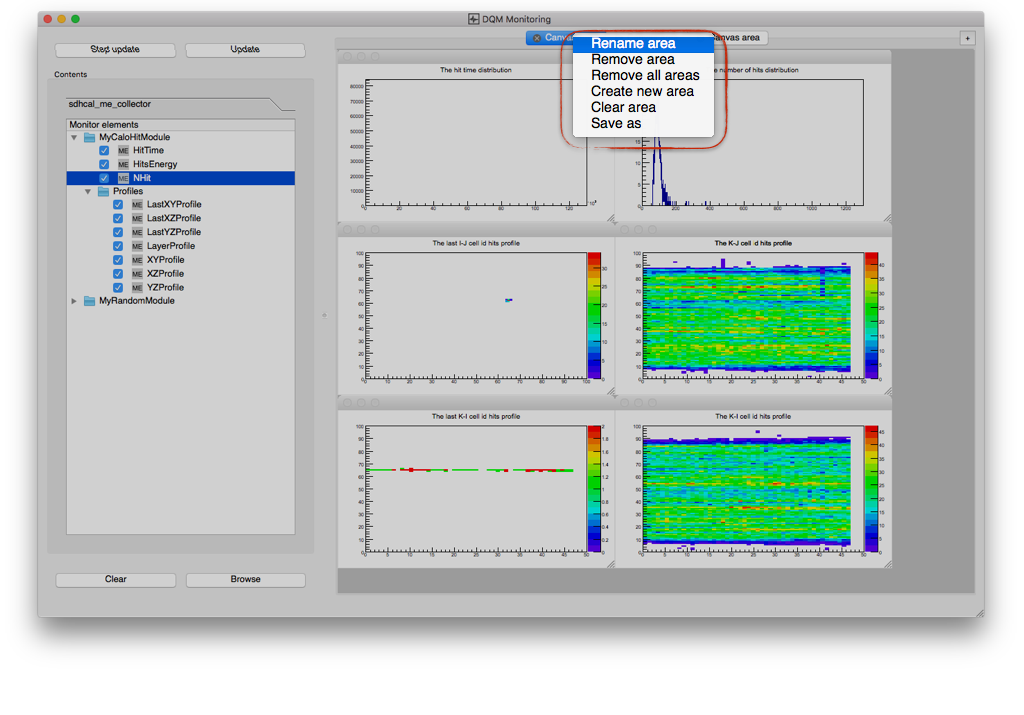
\includegraphics[width=0.8\textwidth]{figs/MonitoringGui/MG_TabsMenu}\end{onlyenv}
         \begin{onlyenv}<4>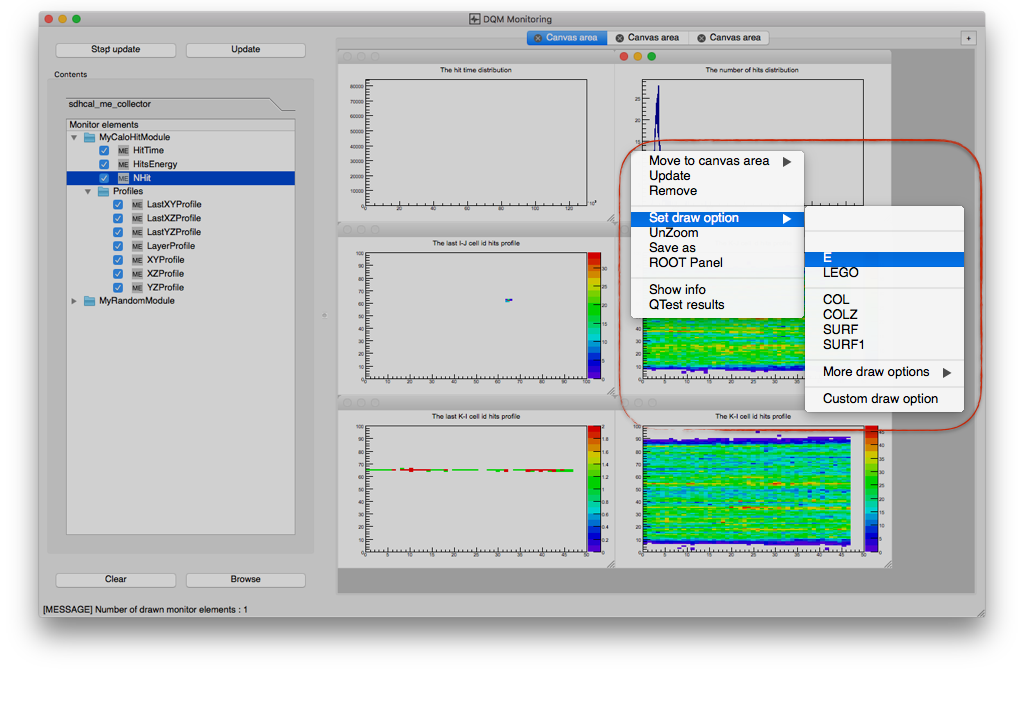
\includegraphics[width=0.8\textwidth]{figs/MonitoringGui/MG_HistosMenu}\end{onlyenv}
         \begin{onlyenv}<5>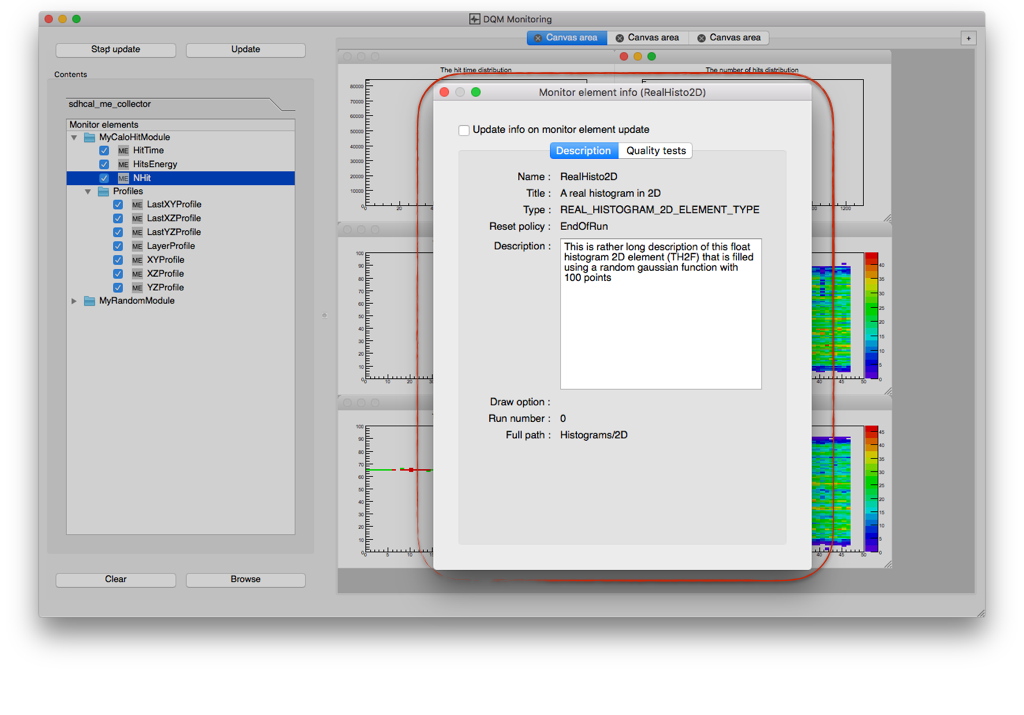
\includegraphics[width=0.8\textwidth]{figs/MonitoringGui/MG_HistoInfo}\end{onlyenv}
         \begin{onlyenv}<6>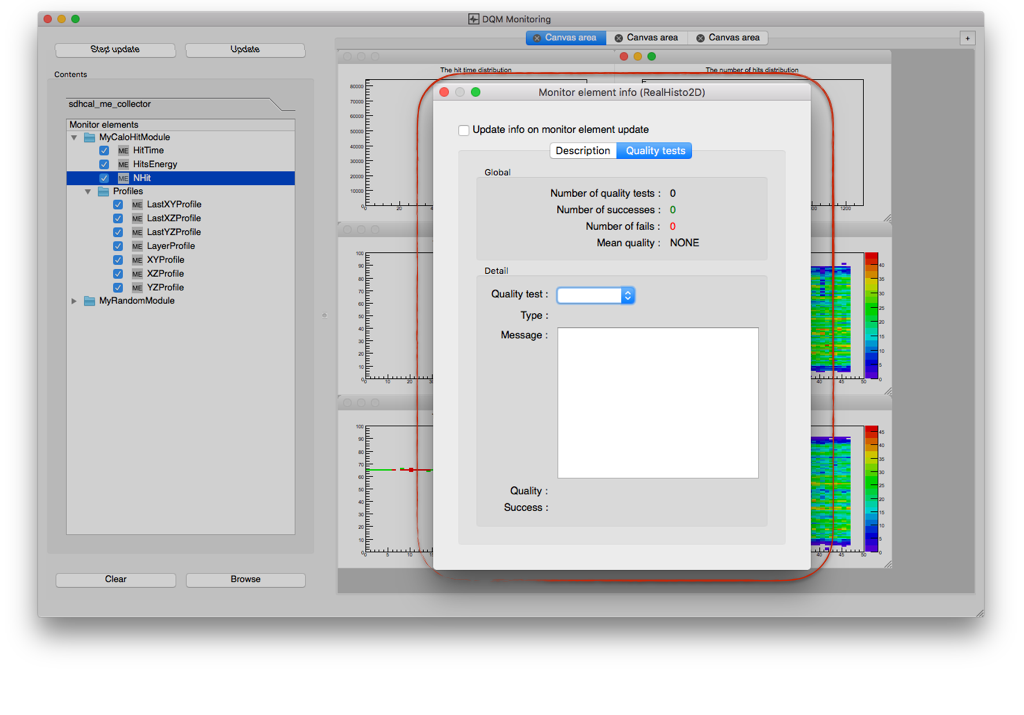
\includegraphics[width=0.8\textwidth]{figs/MonitoringGui/MG_HistoQuality}\end{onlyenv}
         \begin{onlyenv}<7>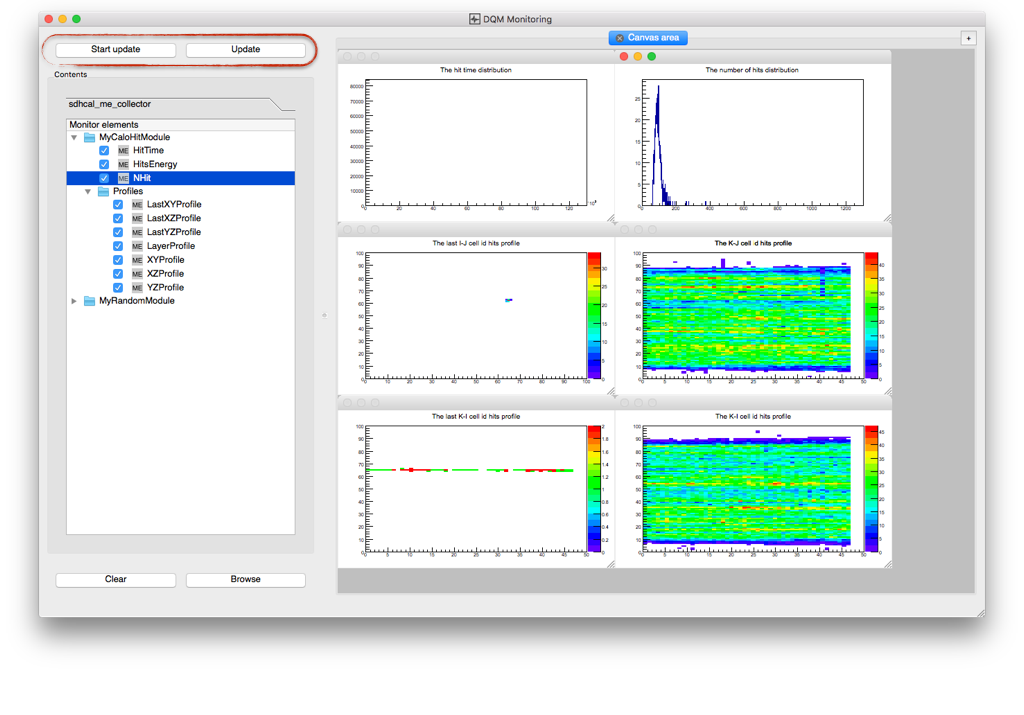
\includegraphics[width=0.8\textwidth]{figs/MonitoringGui/MG_AutoUpdate.png}\end{onlyenv}
      \end{center}


            \vspace{-3em}
       \begin{minipage}{\textwidth}

        \begin{itemize}
         \uncover<1-1>{ \item List of histograms added from Browser }
         \vspace{-1.5em}
       	 \uncover<2->{ \item Multiple canvas area available}
	 \uncover<4->{ \item Real ROOT histograms (Can be fitted, zoomed, etc.) }
       	 \uncover<5-6>{\item Histograms descriptions and Quality}
          \vspace{-1.5em}
       	 \uncover<7->{\item Auto Update }

      \end{itemize}

    \end{minipage}


    \end{overlayarea}

  \end{frame}

  \section{Conclusion and plans}

  %% CONCLUSION %%
  \begin{frame}
  \frametitle{\secname}
  \framesubtitle{Conclusions and plans}

  \begin{block}{Conclusion and plans}
    \begin{itemize}
      \item Independent processes decoupled and linked using networking.
      \item Plugins (modules, data streaming) to configure and run the system.
      \item Tools for data feed in the system from the DAQ (event client interface)
      \item GUIs to control/monitor the system.
      \item Tests are OK but need numbers !
      \item ILCSOFT release ?
    \end{itemize}
  \end{block}

  \begin{block}{Current work and plans}
    \begin{itemize}
      \item Full implementation of SDHCAL DQM
      \item Combined ECAL test-beam -> combined ECAL-HCAL DQM as proof of concept
      \item EUDAQ binding (T. Coates, Sussex, UK)
    \end{itemize}
  \end{block}

  \end{frame}

  \section*{Backups}

  \begin{frame}[containsverbatim]
  \frametitle{\secname}
  \framesubtitle{xdrstream and xdrlcio}

  \begin{itemize}
    \item xdrstream github : \href{https://github.com/DQM4HEP/xdrstream}{\tt https://github.com/DQM4HEP/xdrstream} \\
    Serialization with XDR format to read/write raw data into different devices (file, buffer, socket, user defined) \\
    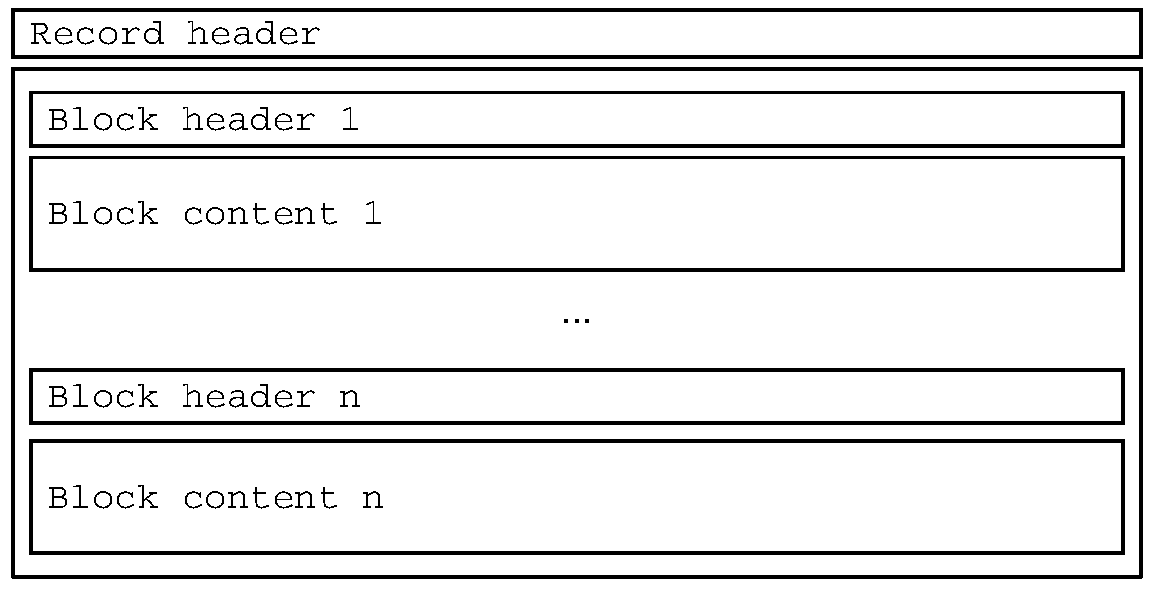
\includegraphics[width=0.4\textwidth]{figs/xdrstream_structure.pdf} \\
    Globally -> SIO implementation :
    \begin{itemize}
      \item without static API (SIO\_blockManager, SIO\_streamManager, etc)
      \item with different device implementation
      \item external standalone package
    \end{itemize}
    For the moment, only buffer implementation (\verb|xdrstream::BufferDevice|)
    \item xdrlcio github : \href{https://github.com/DQM4HEP/xdrlcio}{\tt https://github.com/DQM4HEP/xdrlcio} \\
    LCIO edm serialization using xdrstream. \\
    \textbullet \verb|XdrLcio::writeEvent(const EVENT::LCEvent *pLCEvent,|\\
    ~~\verb|xdrstream::IODevice *const pDevice)| \\
    and \\
    \textbullet \verb|XdrLcio::readNextEvent(xdrstream::IODevice *const pDevice)| \\
    + many useful functions
  \end{itemize}





  \end{frame}



\end{document}
